\chapter{Variabili aleatorie continue e discrete}
\label{ch:teoriasegnali-capitolo5}
\section{Variabili aleatorie}
Si consideri un esperimento aleatorio avente spazio campione $\Omega$, una classe degli eventi $S$ e una legge di probabilità $P(\cdot)$. Si definisce la corrispondenza $X(\omega_i)$ che associa a ciascun risultato $\omega_i\in\Omega$ un unico numero reale $a\in\R$.

Se l'insieme dei risultati di un esperimento aleatorio per i quali è verificata la disuguaglianza $X(\omega)\leq a$ è un evento, $\forall a\in\R$, si dice che $X$ è una \textsc{variabile aleatoria}\index{variabile aleatoria}.

Tale definizione di variabile aleatoria modella un esperimento che ha un risultato numerico non prevedibile a priori ed è derivato da una operazione di misura. Ripetendo l'esperimento si otterrà un insieme di valori che rappresenta la variabile aleatoria.\\

\begin{figure}[ht]
	\centering
	\subfloat[]{\begin{tikzpicture}[scale=.7]\begin{axis}[axis lines=middle,no markers,enlargelimits,xtick={0},ytick={0},xlabel=\(x\),ylabel=\(F_X(x)\)]
		\addplot [very thick] gnuplot [raw gnuplot] {
			% from http://tex.stackexchange.com/a/341886
			set samples 50;
			cdfn(x,mu,sd) = 0.5 * ( 1 + erf( (x-mu)/sd/sqrt(2)) );
			pdfn(x,mu,sd) = 1/(sd*sqrt(2*pi)) * exp( -(x-mu)**2 / (2*sd**2) );
			tpdfn(x,mu,sd,a,b) = pdfn(x,mu,sd) / ( cdfn(b,mu,sd) - cdfn(a,mu,sd) );
			plot [x=-15:9] tpdfn(x,9,10,-10,10)
		};
	\end{axis}\end{tikzpicture}} \qquad
	\subfloat[]{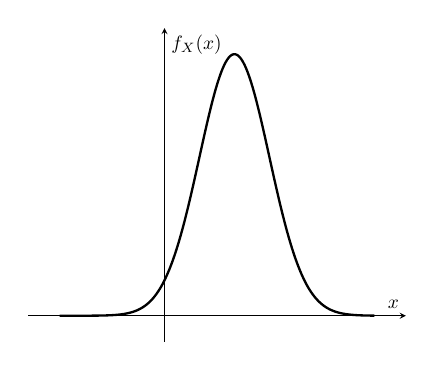
\begin{tikzpicture}[scale=.7]\begin{axis}[axis lines=middle,no markers,enlargelimits,xtick={0},ytick={0},xlabel=\(x\),ylabel=\(f_X(x)\)]
		\addplot [very thick,samples=200,domain=-3:6] {1/(1*sqrt(2*pi))*exp(-((x-2)^2)/(2*1^2))};
	\end{axis}\end{tikzpicture}} \\
	\subfloat[]{\begin{tikzpicture}[scale=.7]\begin{axis}[axis lines=middle,no markers,enlargelimits,xtick={0},ytick={0},xlabel=\(x\),ylabel=\(F_X(x)\)]
		\addplot [very thick] coordinates {(0,0) (1,0) (1,.1) (2,.1) (2,.2) (3,.2) (3,.4) (4,.4) (4,.7) (5,.7) (5,.8) (6,.8) (6,.9) (7,.9) (7,.95) (8,.95) (8,.97) (9,.97) (9,1) (10,1)};
	\end{axis}\end{tikzpicture}} \qquad
	\subfloat[]{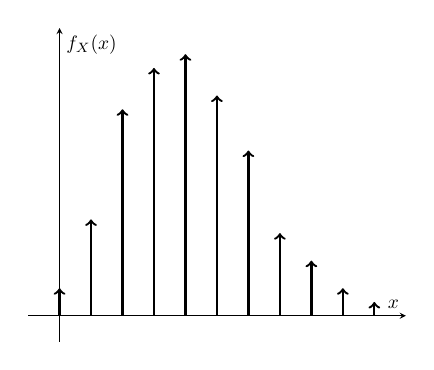
\begin{tikzpicture}[scale=.7]\begin{axis}[axis lines=middle,no markers,enlargelimits,xtick={0},ytick={0},xlabel=\(x\),ylabel=\(f_X(x)\)]
		\addplot [very thick,->] coordinates {(0,0) (0,.02)};
		\addplot [very thick,->] coordinates {(1,0) (1,.07)};
		\addplot [very thick,->] coordinates {(2,0) (2,.15)};
		\addplot [very thick,->] coordinates {(3,0) (3,.18)};
		\addplot [very thick,->] coordinates {(4,0) (4,.19)};
		\addplot [very thick,->] coordinates {(5,0) (5,.16)};
		\addplot [very thick,->] coordinates {(6,0) (6,.12)};
		\addplot [very thick,->] coordinates {(7,0) (7,.06)};
		\addplot [very thick,->] coordinates {(8,0) (8,.04)};
		\addplot [very thick,->] coordinates {(9,0) (9,.02)};
		\addplot [very thick,->] coordinates {(10,0) (10,.01)};
	\end{axis}\end{tikzpicture}} \\
	\subfloat[]{\begin{tikzpicture}[scale=.7]\begin{axis}[axis lines=middle,no markers,enlargelimits,xtick={0},xlabel=\(x\),ylabel=\(F_X(x)\)]
		\addplot [very thick] gnuplot [raw gnuplot] {
			% from http://tex.stackexchange.com/a/341886
			set samples 50;
			cdfn(x,mu,sd) = 0.5 * ( 1 + erf( (x-mu)/sd/sqrt(2)) );
			pdfn(x,mu,sd) = 1/(sd*sqrt(2*pi)) * exp( -(x-mu)**2 / (2*sd**2) );
			tpdfn(x,mu,sd,a,b) = pdfn(x,mu,sd) / ( cdfn(b,mu,sd) - cdfn(a,mu,sd) );
			plot [x=-15:2] tpdfn(x,9,10,-10,10);
			replot [x=2:9] tpdfn(x,9,10,-10,10)+0.05;
		};
		\addplot [very thick] coordinates {(2,0.092) (2,0.1425)};
	\end{axis}\end{tikzpicture}} \qquad
	\subfloat[]{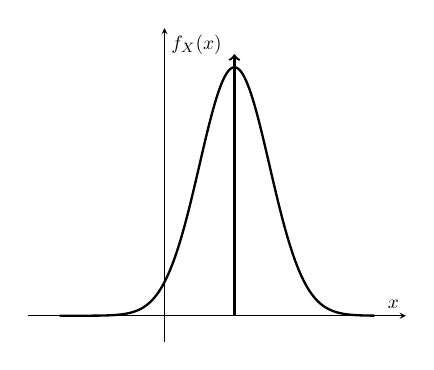
\begin{tikzpicture}[scale=.7]\begin{axis}[axis lines=middle,no markers,enlargelimits,xtick={0},ytick={0},xlabel=\(x\),ylabel=\(f_X(x)\)]
		\addplot [very thick,samples=200,domain=-3:6] {1/(1*sqrt(2*pi))*exp(-((x-2)^2)/(2*1^2))};
		\addplot [very thick,->] coordinates {(2,0) (2,.42)};
	\end{axis}\end{tikzpicture}}
	\caption{Funzioni distribuzione e densità di probabilità per una variabile aleatoria continua, discreta e mista.}
\end{figure}

\section{Funzione distribuzione di probabilità}
Si vuole ora stabilire come trasferire la legge di probabilità sugli eventi alle variabili aleatorie che vi associa numeri sull'asse reale.

Si definisce \textsc{funzione distribuzione di probabilità}\index{variabile aleatoria!funzione distribuzione di probabilità} di una variabile aleatoria $X$ la funzione che associa per un fissato valore reale $x$ il valore della probabilità dell'evento $\lbrace X\leq x\rbrace$, ovvero ne descrive il suo comportamento statistico:
\begin{equation}
\label{eq:funz_dist_prob}
	F_X(x)=P(X\leq x)
\end{equation}

\paragraph{Proprietà funzione distribuzione di probabilità}
\begin{enumerate}
\item $0\leq F_X(x)\leq 1$
\item $\lim\limits_{x\to+\infty}F_X(x)=1$
\item $\lim\limits_{x\to-\infty}F_X(x)=0$
\item $F_X$ è monotona non decrescente:
\[
	x_1<x_2\implies F_X(x_1)\leq F_X(x_2)
\]
\item $F_X$ è continua a destra:
\[
	\lim\limits_{h\to 0^+}{F_X(x+h)}=F_X(x)
\]
\item se $F_X$ presenta discontinuità di prima specie in $\bar{x}$ la probabilità dell'evento $X=\bar{x}$ è pari alla differenza tra limite destro e sinistro
\[
	P(X=\bar{x})=\lim\limits_{h\to 0^+}{F_X(x+h)} - \lim\limits_{h\to 0^-}{F_X(x+h)}
\]
\item la probabilità dell'evento $a < X \leq b$:
\[
	P(a<X\leq b)=F_X(b)-F_X(a)
\]
\end{enumerate}

Le variabili aleatorie possono essere \emph{continue}, \emph{discrete} o \emph{miste} in base alla continuità della funzione distribuzione di probabilità $F_X(x)$.

Per una variabile aleatoria discreta la funzione di distribuzione di probabilità è continua a tratti: $F_X(x)=\sum_k P(X=x_k)\step{(x-x_k)}$, infatti la probabilità è concentrata in “masse” di probabilità $p_k=P(X=x_k)$ in corrispondenza dei punti di discontinuità $x_k$.

Una variabile aleatoria continua ha la funzione distribuzione di probabilità continua, ovvero la probabilità che la variabile aleatoria assuma un particolare valore $P(X=\bar{x})$ è infinitesima.

\section{Funzione densità di probabilità}
Si può dare una definizione alternativa di variabile aleatoria legata alla \textsc{funzione densità di probabilità}\index{variabile aleatoria!funzione densità di probabilità}
\begin{equation}
\label{eq:funz_dens_prob}
	f_X(x)=\deriv{F_X(x)}{x}
\end{equation}
dove la funzione di distribuzione di probabilità
\begin{equation}
	F_X(x)=\intd{-\infty}{x}{f_X(\alpha)}{\alpha}
\end{equation}

\paragraph{Proprietà funzione densità di probabilità}
\begin{enumerate}
\item $f_X(x)\geq 0$ perché $F_X(x)$ è monotona crescente
\item $P(a<X\leq b)=F_X(b)-F_X(a)=\intd{a}{b}{f_X(x)}{x}$
\item $\lim\limits_{x\to\pm\infty}f_X(x)=0$
\item $\intinf{f_X(x)}{x}=1$ in quanto rappresenta la probabilità di un evento certo
\item $P(x<X\leq x+\Delta x)=\intd{x}{x+\Delta x}{f_X(\alpha)}{\alpha}\cong f_X(x)\Delta x$
\end{enumerate}

Per una variabile aleatoria discreta la densità di probabilità è concentrata in impulsi
\begin{equation}
	f_X(x)=\sum_k P(X=x_k) \delta(x-x_k)
\end{equation}

Se la variabile aleatoria è continua la densità di probabilità è distribuita con continuità.
Se la variabile aleatoria è mista coesistono le due condizioni.

\section{Operazioni su variabili aleatorie}
Data una variabile aleatoria $X$ è possibile ottenere una nuova variabile aleatoria che apporti trasformazioni a $X$: $Y=g(X)$. Essa ha funzione distribuzione di probabilità
\begin{equation}
	F_Y(y)=P(Y\leq y)=P(g(X)\leq y)
\end{equation}
Nel dominio $D_Y=\left\lbrace x\mid g(x)\leq y\right\rbrace$ è possibile calcolare la funzione distribuzione di probabilità $F_Y(y)=\int_{D_Y}{f_X(x)\diff x}$ e la funzione densità di probabilità $f_Y(y)=\deriv{F_Y(y)}{y}$

Nel caso in cui la funzione $g(\cdot)$ sia monotona strettamente crescente o strettamente decrescente è possibile definire la sua inversa $g^{-1}(\cdot)$. Di conseguenza nel caso di $g(\cdot)$ strettamente crescente
\[
	F_Y(y)=P(Y\leq y)=P(g(X)\leq y)=P(X\leq g^{-1}(y))=F_X(g^{-1}(y))\implies
\]
\begin{equation}
	f_Y(y)=f_X(g^{-1}(y))\cdot\deriv{g^{-1}(y)}{y}=\restrict{\frac{f_X(x)}{g'(x)}}{x=g^{-1}(y)}
\end{equation}
Nel caso di funzione $g(\cdot)$ strettamente decrescente $g(x)\leq y\iff x>g^{-1}(y)$
\[F_Y(y)=P(Y\leq y)=P(g(X)\leq y)=P(X>g^{-1}(y))=1-F_X(g^{-1}(y))\implies
\]
\begin{equation}
	f_Y(y)=f_X(g^{-1}(y))\cdot-\deriv{g^{-1}(y)}{y}=\restrict{-\frac{f_X(x)}{g'(x)}}{x=g^{-1}(y)}
\end{equation}
In generale
\begin{equation}
	F_Y(y)=\int\limits_{D_Y}{\frac{f_X(x)}{\abs{g'(x)}}\diff x}
\end{equation}
Si osservi l'integrale per $g'(x)=0$ e anche per $f_X(x)=0$ quando sono costanti sia $F_X(x)$ che $g(x)$.

\section{Indici statistici di variabile aleatoria}
Il massimo di informazione che si può trarre da un esperimento aleatorio è la funzione densità di probabilità che caratterizza la variabile aleatoria.
Quando non si conosce questa funzione è comunque possibile determinare dei parametri statistici che permettono di descriverne alcune proprietà.\\

Il più importante parametro statistico è il \textsc{valor medio}\index{valor medio} $\mu_X$ di v.a. continua $X$:
\begin{equation}
\label{eq:v_a_media}
	\mu_X=\intinf{x f_X(x)}{x}
\end{equation}
Per variabile aleatoria discreta si ha $f_X(x)=\sum_k p_k\delta(x-x_k)$, il valor medio
\begin{equation}
\label{eq:v_a_discreta_media}
	\mu_X=\intinf{x f_X(x)}{x}=\sum_k p_k \intinf{x \delta(x-x_k)}{x}=\sum_k x_k p_k
\end{equation}

\`E possibile calcolare il valor medio $\mu_Y$ di funzione trasformata di v.a. $Y=g(X)$ introducendo l'\textsc{operatore aspettazione}\index{operatore!aspettazione}
\begin{equation}
	\E{g(X)}=\intinf{g(x)f_X(x)}{x}
\end{equation}
che nel caso della media assume la semplice relazione $\mu_X=\E{X}$.

L'operatore valor medio gode della proprietà di linearità, data dall'integrale, per cui
\begin{equation}
	\E{a\cdot g(X)+b\cdot h(X)}=a \E{g(X)}+b \E{h(X)}
\end{equation}

Per variabile aleatoria $Y=g(X)$ ottenuta da trasformazione si ha la notevole semplificazione di non dover calcolare la funzione densità di probabilità $f_Y$ nota $f_X$.
Per il \textsc{teorema del valor medio} si può calcolare direttamente il valor medio
\begin{equation}
\label{eq:teo_valor_medio}
	\mu_Y=\E{Y}=\E{g(X)}=\intinf{g(x) f_X(x)}{x}
\end{equation}

Due variabili aleatorie possono avere lo stesso valor medio pur avendo distribuzioni di probabilità differenti. Si quantifica questo indice statistico introducendo il parametro \textsc{varianza}\index{varianza} di variabile aleatoria continua definita come
\begin{equation}
\label{eq:v_a_varianza}
	\sigma^2_X=\E{(X-\mu_X)^2}=\intinf{(x-\mu_X)^2 f_X(x)}{x}
\end{equation}

La varianza di variabile aleatoria discreta
\begin{equation}
\label{eq:v_a_varianza_discreta}
	\sigma^2_X=\E{(X-\mu_X)^2}=\sum_k {(x-\mu_X)^2 p_k}
\end{equation}

Una misura di quanto sia dispersa la probabilità attorno alla media è data dalla \textsc{deviazione standard}\index{deviazione standard} $\sigma_X$, la radice quadrata della varianza.\\

Si definisce \textsc{momento di ordine $k$} l'aspettazione della potenza $k$ di v.a.
\begin{equation}
	\E{X^k}=\intinf{x^k f_X(x)}{x}
\end{equation}

Nel caso particolare $k=2$ si ha l'indice \textsc{valore quadratico medio}\index{valore quadratico medio} o \textsc{potenza statistica} di v.a.
\begin{equation}
\label{eq:v_a_valore_quad_medio}
	m^2_X=\E{X^2}=\intinf{x^2 f_X(x)}{x}
\end{equation}
\begin{nota}
	Il valor quadratico medio è associato alla potenza del segnale, un parametro importante per il dimensionamento di un sistema di telecomunicazioni.
\end{nota}
Varianza e potenza sono legate dalla relazione
\begin{equation}
	\begin{split}
		\sigma^2_X&=\E{(X-\mu_X)^2}=\E{X^2-2X\mu_X+\mu^2_X}=\\
		&=\E{X^2}-2\E{X}\mu_X+\mu^2_X=m^2_X-2\mu^2_X+\mu^2_X=\\
		&=m^2_X-\mu^2_X
	\end{split}
\end{equation}
quindi $\E{X^2}=m^2_X=\sigma^2_X+\mu^2_X$

\section{Funzione generatrice dei momenti}
Per il calcolo degli indici statistici di variabili aleatorie più complesse ci si avvale della \textsc{funzione generatrice dei momenti}\index{funzione generatrice dei momenti}, definita come aspettazione della variabile aleatoria trasformata $\e{t X}$:
\begin{equation}
	\begin{split}
		G_X(t)&=\E{\e{t X}}=\intinf{\e{t x}f_X(x)}{x}=\\
\intertext{sviluppando in serie di Taylor l'esponenziale}
		&=\E{1+x t+\frac{(x t)^2}{2}+\frac{(x t)^3}{3!}+\dots+\frac{(x t)^k}{k!}}=\sum_{k=0}^{+\infty}{\frac{\E{x^k}}{k!}t^k}
	\end{split}
\end{equation}

Si definiscono i momenti di ordine $k$ come derivata della funzione generatrice calcolata in $t=0$.

\begin{description}
\item[Momento del primo ordine (valor medio)]
\begin{equation}
	\restrict{\deriv{G_X(t)}{t}}{t=0}=\E{X}=\mu_X
\end{equation}
\item[Momento del secondo ordine (potenza)]
\begin{equation}
	\restrict{\deriv[2]{G_X(t)}{t}}{t=0}=\E{X^2}
\end{equation}
\item[Momendo di ordine $k$]
\begin{equation}
	\restrict{\deriv[k]{G_X(t)}{t}}{t=0}=\E{X^k}
\end{equation}
\end{description}

\section{Variabile aleatoria uniforme}
La \textsc{variabile aleatoria uniforme}\index{variabile aleatoria!uniforme} presenta una densità di probabilità costante nell'intervallo $[a,b]$ e zero altrove. Dovendo sottendere un'area unitaria si ha un rettangolo di altezza costante $1/(b-a)$, base $(b-a)$ centrato in $(b+a)/2$
\begin{equation}
	f_X(x)=\begin{cases}
		0&x\leq a\\ 
		\frac{1}{b-a}&a<x\leq b\\
		0&x>b
	\end{cases}
	\quad
	f_X(x)=\frac{1}{b-a}\rect{\frac{x-\frac{b+a}{2}}{b-a}}
\end{equation}
La funzione distribuzione essendone l'integrale ha la definizione di una rampa
\begin{equation}
	F_X(x)=\begin{cases}
		0&x\leq a\\
		\frac{x-a}{b-a}&a<x\leq b\\
		1&x>b
	\end{cases}
\end{equation}
\begin{figure}[!ht]
	\centering
	\subfloat[][$f_X(x)$]{
		\begin{tikzpicture}[scale=.7]
			\begin{axis}[axis lines=middle,no markers,enlargelimits,xscale=1.2,xtick={1,2,3},xticklabels={$a$,$\frac{b+a}{2}$,$b$},ytick={2},yticklabels={$\frac{1}{b-a}$},xlabel={$x$}]
			\addplot [very thick] coordinates{(-1,0)(1,0)(1,2)(3,2)(3,0)(4,0)};
			\end{axis}
		\end{tikzpicture}}\qquad
	\subfloat[][$F_X(x)$]{
		\begin{tikzpicture}[scale=.7]
			\begin{axis}[axis lines=middle,no markers,enlargelimits,xscale=1.2,xtick={1,2,3},xticklabels={$a$,$\frac{b+a}{2}$,$b$},ytick={1},xlabel={$x$}]
			\addplot [very thick] coordinates{(-1,0)(1,0)(3,1)(4,1)};
			\end{axis}
		\end{tikzpicture}}
	\caption{Variabile aleatoria uniforme}
\end{figure}

\begin{description}
\item[Valor medio]
\[\mu_X=\intd{a}{b}{\frac{1}{b-a}x}{x}=\frac{1}{b-a}\bound{a}{b}{\frac{x^2}{2}}=\frac{b+a}{2}
\]
\item[Valor quadratico medio] 
\[\E{X^2}=\intd{a}{b}{\frac{1}{b-a}x^2}{x}=\frac{1}{b-a}\bound{a}{b}{\frac{x^3}{3}}=\frac{1}{3}\frac{b^3-a^3}{b-a}=\frac{b^2+a b+a^2}{3}
\]
\item[Varianza]
\[\sigma^2_X=\E{X^2}-\mu^2_X=\frac{b^2+a b+a^2}{3}-\left(\frac{b+a}{2}\right)^2=\frac{(b-a)^2}{12}
\]
\item[Deviazione standard]
\[\sigma_X=\frac{b-a}{2\sqrt{3}}
\]
\item[Deviazione standard normalizzata]
\[\frac{\sigma_X}{\mu_X}=\frac{\frac{b-a}{2\sqrt{3}}}{\frac{b+a}{2}}=\frac{b-a}{b+a}\frac{1}{\sqrt{3}}
\]
\end{description}

\section{Variabile aleatoria esponenziale}
La \index{variabile aleatoria!esponenziale}\textsc{variabile aleatoria continua esponenziale} unilatera con parametro $\lambda>0$ ha una funzione densità di probabilità che parte con una discontinuità in $x=0$ e decresce esponenzialmente a zero. Utile a modellare i tempi di intercorrenza tra richieste di un servizio, problemi di affidabilità e calcolo del rischio. La variabile aleatoria esponenziale è una variabile aleatoria a coda lunga, dove la coda indica eventi rari trascurabili, caratteristica che aiuta a dimensionare i sistemi.
\begin{equation}
	f_X(x)=\lambda\e{-\lambda x}\step(x)
\end{equation}
\begin{equation}
	F_X(x)=\intd{-\infty}{x}{f_X(\alpha)}{\alpha}=\intd{-\infty}{x}{\lambda\e{-\lambda \alpha}}{\alpha}=1-\e{-\lambda x}
\end{equation}
\begin{figure}[!ht]
	\centering
	\subfloat[][$f_X(x)=\lambda\e{-\lambda x}$]{
		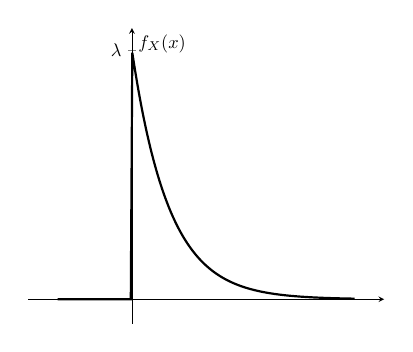
\begin{tikzpicture}[scale=.66]
			\begin{axis}[axis lines=middle,no markers,enlargelimits,xtick={0},ytick={0,2},yticklabels={0,$\lambda$},ylabel={$f_X(x)$}]
			\addplot [very thick,domain=-1:3,samples=200] {x>0?2*exp(-2*x):0};
			\end{axis}
		\end{tikzpicture}}\qquad
	\subfloat[][$F_X(x)=1-\e{-\lambda x}$]{
		\begin{tikzpicture}[scale=.66]
			\begin{axis}[axis lines=middle,no markers,enlargelimits,xtick={0},ytick={0,1},ylabel={$F_X(x)$}]
			\addplot [very thick,domain=-1:3,samples=100] {x>0?1-exp(-2*x):0};
			\end{axis}
		\end{tikzpicture}
	}
	\caption{Variabile aleatoria esponenziale}
\end{figure}

\begin{flushleft}
Calcolo degli indici statistici:
\end{flushleft}
\begin{description}
\item[Valor medio]
\begin{equation}
\begin{split}
	\mu_X&=\intinf{x f_X(x)}{x}=\intd{0}{+\infty}{x \lambda\e{-\lambda x}}{x}=\\
\intertext{integrando per parti $\int{u \diff v}=u v-\int{v\diff u}, u=\lambda x$, $\diff u=\lambda\diff x$, $\diff v=\e{-\lambda x}\diff x$, $v=-\frac{1}{\lambda}\e{-\lambda x}$}
	&=\bound{0}{+\infty}{-x\e{-\lambda x}}+\intd{0}{+\infty}{\e{-\lambda x}}{x}=\frac{1}{\lambda} 	\qquad\text{essendo} \intd{0}{+\infty}{\lambda\e{-\lambda x}}{x}=1
\end{split}
\end{equation}
\item[Potenza]
\begin{equation}
\begin{split}
	\E{X^2}&=\intinf{x^2 f_X(x)}{x}=\intd{0}{+\infty}{\lambda x^2\e{-\lambda x}}{x}=\\
\intertext{integrando per parti $u=x^2$, $\diff u=2x\diff x$, $\diff v=\lambda\e{-\lambda x}$, $v=-\e{-\lambda x}$}
	&=\bound{0}{+\infty}{-x^2\e{-\lambda x}}+\frac{2}{\lambda}\underbrace{\intd{0}{+\infty}{x \lambda\e{-\lambda x}}{x}}_{{\mu_X}={\frac{1}{\lambda}}}=\frac{2}{\lambda^2}
\end{split}
\end{equation}
\item[Varianza]
\[
	\sigma^2_X=\E{X^2}-\mu^2_X=\frac{2}{\lambda^2}-\frac{1}{\lambda^2}=\frac{1}{\lambda^2}
\]
\item[Deviazione standard]
\[
	\sigma_X=\frac{1}{\lambda}=\mu_X
\]
\item[Deviazione standard normalizzata dalla media] \[
	\frac{\sigma_X}{\mu_X}=1
\]
\end{description}

\section{Variabile aleatoria discreta di Poisson}
La \index{variabile aleatoria!di Poisson}\textsc{variabile aleatoria discreta di Poisson} modella le richieste di servizio o il conteggio per arrivi indipendenti in un intervallo di tempo $T$ e con un parametro di intensità $\Lambda>0$ in istanti di tempo discreti (valori interi non negativi). La funzione densità di probabilità (di massa) $f_X(x)=\sum_k p_k \delta(x-k)$ ha espressione
\begin{equation}
	f_X(x)=\sum_{k=0}^{+\infty}{\frac{(\Lambda T)^k}{k!}\e{-\Lambda T}\delta(x-k)}
\end{equation}
La funzione distribuzione di probabilità (di massa) $F_X(x)=\sum_k p_k \step(x-k)$ ha espressione
\begin{equation}
	F_X(x)=\sum_{k=0}^{+\infty}{\frac{(\Lambda T)^k}{k!}\e{-\Lambda T}\step(x-k)}
\end{equation}
con masse di probabilità $p_k=\frac{(\Lambda T)^k}{k!}\e{-\Lambda T}$.

\begin{flushleft}
Calcolo degli indici statistici:
\end{flushleft}
\begin{description}
\item[Valor medio]
\begin{equation}
\begin{split}
	\mu_X&=\sum_{k=0}^{+\infty}{k p_k}=\sum_{k=0}^{+\infty}{k \frac{(\Lambda T)^k}{k!}\e{-\Lambda T}}=\sum_{k=1}^{+\infty}{\frac{(\Lambda T)^k}{(k-1)!}\e{-\Lambda T}}=\\
	&=\Lambda T \e{-\Lambda T} \sum_{k=1}^{+\infty}{\frac{(\Lambda T)^{k-1}}{(k-1)!}}=\Lambda T \e{-\Lambda T}\sum_{z=0}^{+\infty}{\frac{(\Lambda T)^z}{z!}}=\Lambda T \e{-\Lambda T}\e{\Lambda T}=\\
	&=\Lambda T
\end{split}
\end{equation}
\item[Potenza]
\begin{equation}
\begin{split}
	\E{X^2}&=\sum_{k=0}^{+\infty}{k^2 p_k}=\sum_{k=0}^{+\infty}{k^2 \frac{(\Lambda T)^k}{k!}\e{-\Lambda T}}=\e{-\Lambda T}\sum_{k=0}^{+\infty}{k\frac{(\Lambda T)^k}{(k-1)!}}=\\
	&=\e{-\Lambda T}\sum_{k=1}^{+\infty}{k\frac{(\Lambda T)^{z-1}}{(k-1)!}\Lambda T}=
	\e{-\Lambda T}\sum_{k=1}^{+\infty}{(k-1+1)\frac{\Lambda T(\Lambda T)^{z-1}}{(k-1)!}}=\\
	&=\e{-\Lambda T}\left[\sum_{k=1}^{+\infty}{(k-1)\frac{\Lambda T(\Lambda T)^{z-1}}{(k-1)!}} + \sum_{k=1}^{+\infty}{\frac{\Lambda T(\Lambda T)^{z-1}}{(k-1)!}}\right]=\\
	&=\e{-\Lambda T}\left[\sum_{z=0}^{+\infty}{z\frac{\Lambda T(\Lambda T)^z}{z!}} + \Lambda T\e{\Lambda T}\right]=\\
	&=\e{-\Lambda T}\left[\sum_{z=1}^{+\infty}{\frac{\Lambda T(\Lambda T)^{z-1}}{(z-1)!}} + \Lambda T\e{\Lambda T}\right]=\\
	&=\e{-\Lambda T}\left[(\Lambda T)^2 \e{\Lambda T} + \Lambda T\e{\Lambda T}\right]=\\
	&=(\Lambda T)^2 + \Lambda T
\end{split}
\end{equation}
\end{description}

Gli stessi indici possono essere calcolati più agevolmente con la funzione generatrice dei momenti:
\begin{equation}
	G_X(t)=\sum_{k=0}^{+\infty}{\e{t x}p_k\delta(x-k)}=\sum_{k=0}^{+\infty}{\e{t k}\frac{(\Lambda T)^k}{k!}\e{-\Lambda T}}=\sum_{k=0}^{+\infty}{\frac{(\e{t}\Lambda T)^k}{k!}\e{-\Lambda T}}=\e{-\Lambda T}\e{\Lambda T\e{t}}
\end{equation}

\begin{description}
\item[Valor medio (momento del primo ordine)]
\begin{equation}
\begin{split}
	\mu_X&=\restrict{\deriv{G_X(t)}{t}}{t=0}=\restrict{\deriv{\e{-\Lambda T}\e{\Lambda T\e{t}}}{t}}{t=0}=\restrict{\e{-\Lambda T}{\Lambda T}\e{t}\e{\Lambda T\e{t}}}{t=0}=\Lambda T \e{-\Lambda T}\e{\Lambda T}=\\
	&=\Lambda T
\end{split}
\end{equation}

\item[Potenza (momento del secondo ordine)]
\begin{equation}
\begin{split}
	\E{X^2}&=\restrict{\deriv[2]{G_X(t)}{t}}{t=0}=
	\restrict{\deriv{\e{-\Lambda T}{\Lambda T}\e{t}\e{\e{t}\Lambda T}}{t}}{t=0}=
	\restrict{\e{-\Lambda T}{\Lambda T}\deriv{\e{t}\e{\e{t}\Lambda T}}{t}}{t=0}=\\
	&={\e{-\Lambda T}\Lambda T}\restrict{\left[\e{t}\e{\e{t}\Lambda T}+\e{t}\e{\e{t}\Lambda T}{\e{t}\Lambda T}\right]}{t=0}=\\
	&={\e{-\Lambda T}\Lambda T}[\e{\Lambda T}+\e{\Lambda T}{\Lambda T}]=\\
	&=(\Lambda T)^2+\Lambda T
\end{split}
\end{equation}
\end{description}

\section{Variabile aleatoria binomiale o di Bernoulli}
Variabile aleatoria discreta applicata ad esperimenti ripetuti di \index{variabile aleatoria!di Bernoulli}\textsc{Bernoulli}, indipendenti tra loro, che possono dare due soli possibili risultati, successo con probabilità $p$ e insuccesso con probabilità $1-p$. La variabile binomiale conta il numero di successi.
La funzione densità di probabilità (di massa) $f_X(x)=\sum_k p_k \impulse(x-k)$ e la funzione distribuzione di probabilità (di massa) $F_X(x)=\sum_k p_k \step(x-k)$ hanno massa di probabilità data dalla formula binomiale di Bernoulli:
\begin{equation}
	P(X=k)=\binom{n}{k} p^k (1-p)^{n-k}\quad k=0,\dots,n
\end{equation}
Funzione generatrice dei momenti
\begin{equation}
\begin{split}
	G_X(t)=\E{\e{t X}}&=\sum_{k=0}^{n}{\e{t k}\binom{n}{k}p^k(1-p)^{n-k}}=\\
	&=\sum_{k=0}^{n}{\binom{n}{k}(p\e{t})^k(1-p)^{n-k}}=\\
	&=(p\e{t}+1-p)^n
	\end{split}
\end{equation}
\begin{flushleft}
Calcolo degli indici statistici utilizzando la funzione generatrice dei momenti:
\end{flushleft}
\begin{description}
\item[Valor medio]
\begin{equation}
	\mu_X=\restrict{\deriv{G_X(t)}{t}}{t=0}=\restrict{n(p\e{t}+1-p)^{n-1}p\e{t}}{t=0}=n p
\end{equation}
\item[Potenza]
\begin{equation}
\begin{split}
	\E{X^2}&=\restrict{\deriv[2]{G_X(t)}{t}}{t=0}=\restrict{\deriv{np\e{t}(p\e{t}+1-p)^{n-1}}{t}}{t=0}=\\
	&=\restrict{np\e{t}(p\e{t}+1-p)^{n-1}+np\e{t}(n-1)(p\e{t}+1-p)^{n-2}p\e{t}}{t=0}=\\
	&=np+np^2(n-1)=\\
	&=np[p(n-1)+1]
\end{split}
\end{equation}
\item[Varianza]
\begin{equation}
\begin{split}
	\sigma^2_X&=\E{X^2}-\Esp^2[X]=np[p(n-1)+1]-n^2p^2=\\
	&=np+n^2p^2-np^2-n^2p^2=\\
	&=np(1-p)
\end{split}
\end{equation}
\end{description}

\section{Variabile aleatoria geometrica}
La \index{variabile aleatoria!geometrica}\textsc{variabile aleatoria geometrica} è una variabile aleatoria discreta che consente di calcolare la probabilità di ottenere il primo insuccesso dopo aver ottenuto $k$ successi consecutivi quando si effettuano degli esperimenti indipendenti e ripetuti di Bernoulli.
La variabile aleatoria geometrica ha pertanto masse di probabilità
\begin{equation}
	P(X=k)=p^k(1-p)\quad k=0,\dots,\infty
\end{equation}
La funzione generatrice dei momenti
\begin{equation}
\begin{split}
	G_X(t)=\E{\e{t X}}&=\sum_{k=0}^{\infty}{\e{t k}p^k(1-p)}=(1-p)\sum_{k=0}^{\infty}{(p\e{t})^k}=\\
	&=\frac{1-p}{1-p\e{t}}=(1-p)(1-p\e{t})^{-1}
\end{split}
\end{equation}
dove la serie geometrica $\sum_{k=0}^{\infty}{(p\e{t})^k}$ converge in un intorno di $t=0$ dove calcoliamo i momenti.

\begin{description}
\item[Valor medio]
\begin{equation}
	\mu_X=\restrict{\deriv{G_X(t)}{t}}{t=0}=\restrict{(1-p)(-1)(1-p\e{t})^{-2}(-p\e{t})}{t=0}=\frac{p}{1-p}
\end{equation}
\item[Potenza]
\begin{equation}
\begin{split}
	\E{X^2}&=\restrict{\deriv[2]{G_X(t)}{t}}{t=0}=\restrict{\deriv{p(1-p)\e{t}(1-p\e{t})^{-2}}{t}}{t=0}=\\
	&=p(1-p)\restrict{[\e{t}(1-p\e{t})^{-2}+\e{t}2(1-p\e{t})^{-3}p]}{t=0}=\\
	&=p(1-p)[(1-p)^{-2}+2p(1-p)^{-3}]=\\
	&=p(1-p)\frac{(1-p)+2p}{(1-p)^3}=\\
	&=\frac{p(1+p)}{(1-p)^2}
\end{split}
\end{equation}
\item[Varianza]
\begin{equation}
	\sigma^2_X=\E{X^2}-\Esp^2[X]=\frac{p(1+p)}{(1-p)^2}-\frac{p^2}{(1-p)^2}=\frac{p}{(1-p)^2}
\end{equation}
\item[Deviazione standard]
\begin{equation}
	\sigma_X=\frac{\sqrt{p}}{1-p}
\end{equation}
\end{description}

\section{Derivazione e significato delle variabili aleatorie esponenziale e di Poisson}
La variabile aleatoria esponenziale e quella discreta di \index{variabile aleatoria!di Poisson}\textsc{Poisson} modellano esperimenti di richieste di servizio o attesa di eventi indipendenti tra loro. Nell'intervallo di tempo fissato $T$ si vuole calcolare la probabilità che si verifichino un certo numero di eventi, quale sia il tempo di interarrivo, il tempo che intercorre tra due eventi successivi, e il tempo di attesa affinché si verifichi il primo evento a partire da un istante iniziale di riferimento.

\`E possibile derivare la distribuzione di probabilità della v.a. di Poisson studiando il fenomeno sotto alcune ipotesi.

Fissato il periodo $T$ lo si suddivide in $n$ intervallini di durata $\delta T=\frac{T}{n}$. Si prova a descrivere come v.a. di Bernoulli la possibilità che possano verificarsi $k$ eventi nell'intervallo finito $T$, al più un evento per ogni singolo intervallino $\delta T$.
\begin{equation}
\begin{cases}
	P(N(\delta T)=1)&=p\\
	P(N(\delta T)=0)&=1-p
\end{cases}
\end{equation}
\begin{equation}
	P(N(T)=k)=\binom{n}{k}p^k(1-p)^{n-k}
\end{equation}
Detta $\Lambda$ l'intensità del processo di Poisson, si ha che $\Lambda T=n p=\alpha$ è il numero medio di arrivi nell'intervallo di tempo $T$. Tale intensità è caratteristica del processo e non dipende dal numero di intervallini in cui si suddivide $T$. Portando al limite il numero di intervallini, $n\to\infty$ si ha

\begin{equation}
\begin{split}
	P(N(T)=k)&=\binom{n}{k}p^k(1-p)^{n-k}=\lim\limits_{n\to\infty}\binom{n}{k}\left(\frac{\alpha}{n}\right)^k\left(1-\frac{\alpha}{n}\right)^{n-k}=\\
	&=\lim\limits_{n\to\infty}\frac{n!}{k!(n-k)!}\left(\frac{\alpha}{n}\right)^k\left(1-\frac{\alpha}{n}\right)^{n-k}=\\
	&=\frac{\alpha^k}{k!}\lim\limits_{n\to\infty}\underbrace{\frac{n!}{n^k(n-k)!}}_{\to 1}\underbrace{\left(1-\frac{\alpha}{n}\right)^n}_{\to\e{-\alpha}} \underbrace{\left(1-\frac{\alpha}{n}\right)^{-k}}_{\to 1}=\\
	&=\frac{\alpha^k}{k!}\e{-\alpha}=\frac{(\Lambda T)^k}{k!}\e{-\Lambda T}
	\end{split}
\end{equation}

Con $T=1$ si ha la probabilità che nell'unità di tempo si verifichino $k$ eventi.

La probabilità che non capitino eventi vale $P(N(1)=0)=\e{-\Lambda}$.

Si vuole calcolare ora il \emph{tempo di attesa}, ovvero il tempo che bisogna attendere fino al primo evento a partire dall'istante iniziale di osservazione. La distribuzione di probabilità della variabile aleatoria tempo di attesa può essere espressa come probabilità che non sia capitato alcun evento fino al tempo $x$ ovvero $P(\tau>x)=\e{-\Lambda x}$
\begin{equation}
	F_\tau(x)=P(\tau\leq x)=1-P(\tau\geq x)=1-\e{-\Lambda x}
\end{equation}
\begin{equation}
	f_\tau(x)=\Lambda\e{-\Lambda x}
\end{equation}
che risulta essere una funzione di distribuzione di una variabile aleatoria esponenziale.

Si può vedere infatti che se fino ad un tempo $\tau$ non ho eventi il tempo di attesa per il successivo evento è sempre esponenziale, con lo stesso parametro $\Lambda$ (processo fisico privo di memoria):
\[
	P(X>\tau+t_0|X>\tau)=\frac{P(X>\tau+t_0,X>\tau)}{P(X>\tau)}=\frac{P(X>\tau+t_0)}{P(X>\tau)}=\frac{\e{-\Lambda(\tau+t_0)}}{\e{-\Lambda\tau}}=\e{-\Lambda t_0}
\]

Similmente a partire da un istante in cui è capitato un evento si voglia determinare qual è la probabilità che sia $\tau$ il tempo da attendere per l'evento successivo. Per eventi indipendenti il tempo di interarrivo ha distribuzione e densità di probabilità uguali a quelle calcolate per il tempo di attesa, ovvero di una variabile aleatoria esponenziale con parametro $\Lambda$ caratteristica di un sistema privo di memoria.

\begin{nota}
	Nei sistemi ingegneristici la v.a. esponenziale modella la “coda lunga” che tiene conto della probabilità di eventi rari che possono avvenire in un tempo infinito. Nella pratica si utilizza una variabile aleatoria esponenziale troncata, in cui si corregge con un fattore moltiplicativo la funzione densità per ottenere un'area unitaria.
\end{nota}

\begin{esempio}
Il circuito elettrico $RC$ alimentato dal generatore di tensione $V_i$ a partire dall'istante $t=0$ modella un resistore che ha un tempo di guasto aleatorio descritto da variabile aleatoria esponenziale con funzione densità di probabilità esponenziale monolatera
\[
	f_X(x)=\frac{1}{2\alpha}\e{-\frac{x}{2\alpha}}\step(x)\quad\alpha=RC
\]
\begin{figure*}[h]
	\centering
	\begin{circuitikz}[american voltages]
		\draw (0,0)	to[battery,v^>=${V_i}$] (0,3)
		to[switch,l=${t=0}$] (2,3)
		to[opening switch,l=${t=X}$] (4,3)
		to[R, l=${R}$] (6,3)
		to[C, l=${C}$,i>_=${i(t)}$] (6,0) to[short] (0,0)
		(6,0) -- (7,0) to[open,v>=${V_o(t)}$, *-*] (7,3) -- (6,3);
	\end{circuitikz}
\end{figure*}

Qual è la tensione di uscita $V_o(X)$ nel momento del guasto?

Per rispondere bisogna esprimere la funzione densità di probabilità $fV_(v)$ della v.a. $V_o(X)$ trasformata della v.a. tempo di guasto $X$. Il legame tra il tempo e la tensione sul condensatore è  $V_o(t)=V_i(1-\e{-\frac{t}{\alpha}})$.
Si ha così la variabile aleatoria trasformata $V(X)=V_i(1-\e{-\frac{x}{\alpha}})\step(X)$

Per il teorema fondamentale della trasformazione di variabile aleatoria la funzione densità di probabilità si calcola come
\[
	f_V(x)=\restrict{\frac{f_X(x)}{\abs{g'(x)}}}{x=g^{-1}(v)}
\]
dove $g(x)=v=V_i(1-\e{\frac{x}{\alpha}})$, $g'(x)=\frac{V_i}{\alpha}\e{-\frac{x}{\alpha}}$ e $x=g^{-1}(v)=-\alpha\f{\ln}{1-\frac{v}{V_i}}$, sostituendo la $f_X(x)$ si ha
\[
	f_V(v)=\restrict{\frac{\frac{1}{2\alpha}\e{-\frac{x}{2\alpha}}}{\abs{\frac{V_i}{\alpha}\e{-\frac{x}{\alpha}}}}}{x=g^{-1}(v)}=
	\frac{\frac{1}{2\alpha}\e{-\frac{-\alpha\f{\ln}{1-\frac{v}{V_i}}}{2\alpha}}}{\frac{V_i}{\alpha}\e{-\frac{-\alpha\f{\ln}{1-\frac{v}{V_i}}}{\alpha}}}=
	\frac{1}{2 V_I}\frac{\e{\ln\sqrt{\left(1-\frac{v}{V_i}\right)}}}{\e{\f{\ln}{1-\frac{v}{V_i}}}}=
	\frac{1}{2 V_i}\frac{1}{\sqrt{\left(1-\frac{v}{V_i}\right)}}
\]

\begin{figure}[h]
	\centering
	\subfloat[][$f_X(x)$]{
		\begin{tikzpicture}[scale=.8]
			\begin{axis}[axis lines=middle,no markers,enlargelimits,xtick={0},ytick={0,.5},yticklabels={0,$\frac{1}{2\alpha}$},xlabel=$x$,ylabel={$f_X(x)$}]
			\addplot [very thick,domain=-0.5:0,samples=2] {0};
			\addplot [very thick,domain=0:3,samples=200] {0.5*exp(-x)};
			\end{axis}
		\end{tikzpicture}}\qquad
	\subfloat[][$f_V(v)$]{
		\begin{tikzpicture}[scale=.8]
			\begin{axis}[axis lines=middle,no markers,enlargelimits,xtick={1},ytick={0,.5},xticklabels={$V_i$},yticklabels={0,$\frac{1}{2 V_i}$},xlabel=$v$,ylabel={$f_V(v)$}]
			\addplot [very thick,domain=-0.5:0,samples=2] {0};
			\addplot [very thick,domain=0:0.9,samples=200] {0.5/sqrt(1-x)};
			\addplot [very thick,domain=1:1.5,samples=2] {0};
			\end{axis}
		\end{tikzpicture}}
	\caption{Funzione densità di probabilità e sua trasformata}
\end{figure}

\end{esempio}

\section{Variabile aleatoria gaussiana o normale}
La \index{variabile aleatoria!gaussiana}\textsc{variabile aleatoria gaussiana} $X\in\mathcal{N}(\mu_X,\sigma^2_X)$ ha funzione densità di probabilità
\begin{equation}
\label{eq:densita_gaussiana}
	f_X(x)=\frac{1}{\sqrt{2\pi\sigma^2_X}}\;\e{-\tfrac{(x-\mu_X)^2}{2\sigma^2_X}}
\end{equation}
dove, come si dimostra, $\mu_X$ e $\sigma^2_X$ sono il valor medio e la varianza che caratterizzano la variabile aleatoria stessa.
Modella esperimenti che sono la risultante di tanti fenomeni elementari indipendenti.

La variabile aleatoria gaussiana $X_N\in\mathcal{N}(0,1)$ a valor medio nullo e varianza unitaria è detta \textsc{variabile normale standard}
\begin{equation}
\label{eq:densita_normale}
	f_{X_N}(x)=\frac{1}{\sqrt{2\pi}}\;\e{-\tfrac{x^2}{2}}
\end{equation}
Per il teorema fondamentale della trasformazione di variabile aleatoria si ha che la generica variabile gaussiana $X\in\mathcal{N}(\mu_X,\sigma^2_X)$ può essere espressa come trasformazione lineare della variabile aleatoria normale standard $X_N$:
\begin{equation}
	X=\sigma_X\cdot X_N+\mu_X
\end{equation}
\begin{equation}
	f_X(x)=\frac{1}{\sigma_X}\f{f_{X_N}}{\frac{x-\mu_X}{\sigma_X}}=\frac{1}{\sqrt{2\pi\sigma^2_X}}\;\e{-\tfrac{(x-\mu_X)^2}{2\sigma^2_X}}
\end{equation}


\begin{figure}[!ht]
\centering
\begin{tikzpicture}
\begin{axis}[axis x line=middle, axis y line=left,no markers,enlargelimits,xscale=2,xtick={-3,-2,-1,0,1,2,3},xticklabels={$\mu-3\sigma$,$\mu-2\sigma$,$\mu-\sigma$,$\mu$,$\mu+\sigma$,$\mu+2\sigma$,$\mu+3\sigma$},ytick={0.3989},yticklabels={$\frac{1}{\sqrt{2\pi\sigma^2}}$},xlabel=$x$,
after end axis/.code={\draw [thick,decoration={brace,mirror,raise=17pt},decorate]
	(axis cs:-1,0) -- node[below=17pt] {$68,3\%$} (axis cs:1,0);
	\draw [thick,decoration={brace,mirror,raise=35pt,amplitude=5pt},decorate]
	(axis cs:-2,0) -- node[below=37pt] {$95,4\%$} (axis cs:2,0);
	\draw [thick,decoration={brace,mirror,raise=52pt,,amplitude=10pt},decorate]
	(axis cs:-3,0) -- node[below=60pt] {$99,74\%$} (axis cs:3,0);
}
]
\pgfmathsetmacro\valueMu{gauss(0,0,1)}
\pgfmathsetmacro\valueA{gauss(1,0,1)}
\pgfmathsetmacro\valueB{gauss(2,0,1)}
\draw [dashed] (axis cs:0,0) -- (axis cs:0,\valueMu);
\draw [dashed] (axis cs:1,0) -- (axis cs:1,\valueA)
(axis cs:-1,0) -- (axis cs:-1,\valueA);
\draw [dashed] (axis cs:2,0) -- (axis cs:2,\valueB)
(axis cs:-2,0) -- (axis cs:-2,\valueB);
\addplot[very thick,smooth,domain=-4:4] {gauss(x,0,1)};
\end{axis}\end{tikzpicture}
\caption{Funzione densità di probabilità di variabile aleatoria gaussiana}
\end{figure}

La funzione di distribuzione di variabile aleatoria gaussiana non può essere calcolata in forma chiusa, ma può essere calcolata con metodi numerici la funzione di distribuzione di probabilità gaussiana standard
\begin{equation}
	\Phi_{X_N}=\intd{-\infty}{x}{\frac{1}{\sqrt{2\pi}}\;\e{-\tfrac{z^2}{2}}}{z}
\end{equation}
o la sua complementare $Q_{X_N}=1-\Phi_{X_N}$.

La funzione di distribuzione per la variabile aleatoria gaussiana si calcola applicando la trasformazione $X=\sigma_X X_N +\mu_X$ nella funzione di distribuzione di probabilità della variabile aleatoria normale standard
\begin{equation}
	F_X(x)=P(X\leq x)=P(\sigma_X\cdot X_N+\mu_X\leq x)=\f{P}{X_N\leq\frac{x-\mu_X}{\sigma_X}}=\f{\Phi_{X_N}}{\frac{x-\mu_X}{\sigma_X}}
\end{equation}
La probabilità che la v.a. gaussiana assuma valori in un intervallo $[a,b]$ si calcola
\[
	P(a<x\leq b)=F_X(b)-F_X(a)=\f{\Phi_{X_N}}{\frac{b-\mu_X}{\sigma_X}}-\f{\Phi_{X_N}}{\frac{a-\mu_X}{\sigma_X}}
\]
I valori di $\Phi_{X_N}$ sono tabulati o calcolati con le funzioni errore e errore complementare presenti nei calcolatori elettronici
\begin{equation}
	\erf{x}=\frac{2}{\sqrt{\pi}}\intd{0}{x}{\e{-z^2}}{z}
\end{equation}
\begin{equation}
	\erfc{x}=1-\erf{x}=\frac{2}{\sqrt{\pi}}\intd{x}{+\infty}{\e{-z^2}}{z}
\end{equation}
La funzione di distribuzione standard calcolata dalla funzione errore
\begin{equation}
	\Phi(x)=\frac{1}{2}\left(1+\erf{\frac{x}{\sqrt{2}}}\right)
\end{equation}
\begin{equation}
	Q(x)=\frac{1}{2}\erfc{\frac{x}{\sqrt{2}}}
\end{equation}

\begin{figure}[!ht]
	\centering
	\subfloat[][funzione di distribuzione di probabilità v.a. normale standard]{
		\begin{tikzpicture}
			\begin{axis}[axis lines=middle,no markers,enlargelimits,xtick={0},ytick={.5,1},xlabel=$x$,ylabel=$\Phi_{X_N}(x)$]
			\addplot[very thick,smooth] gnuplot[id=erfc]{.5*(1+erf(x/sqrt(2)))};
			\end{axis}
		\end{tikzpicture}}\quad
	\subfloat[][funzione errore e errore complementare]{
		\begin{tikzpicture}
			\begin{axis}[axis lines=middle,no markers,enlargelimits,xtick={0},ytick={-1,1,2},xlabel=$x$]
			\addplot[very thick,smooth] gnuplot[id=erf]{erf(x)} node [above,pos=1,pin={135:$\erf{x}$}] {};
			\addplot[dashed,smooth] gnuplot[id=erf]{erfc(x)} node [below,pos=.33,pin={-135:$\erfc{x}$}] {};
			\end{axis}
		\end{tikzpicture}}
\end{figure}

Si dimostra che l'integrale della funzione densità di probabilità
\[
	S=\intinf{f_X(x)}{x}=1
\]
\begin{proof}[Dim.]
Non avendo $\int\e{-z^2}\diff z$ soluzioni in forma chiusa, si considera che $S^2=1$ e si ha l'integrale doppio
\[
	S^2=\intinf{f_X(x)}{x}\intinf{f_Y(y)}{y}=\intinf{\intinf{\frac{1}{2\pi\sigma^2}\e{-\tfrac{(x-\mu)^2(y-\mu)^2}{2\sigma^2}}}{y}}{x}
\]
Per risolvere l'integrale si applica la trasformazione da variabili cartesiane a variabili polari
\[
	\begin{split}\frac{x-\mu}{\sigma}=\rho\cos{\theta}&\qquad\frac{y-\mu}{\sigma}=\rho\sen{\theta}\\
	\deriv{x}{\rho}=\sigma\cos{\theta}&\qquad\deriv{y}{\rho}=\sigma\sen{\theta}\\
	\deriv{x}{\theta}=-\sigma\rho\sen{\theta}&\qquad\deriv{y}{\theta}=\sigma\rho\cos{\theta}\\
	\diff x\diff y=\abs{J(\rho,\theta)}\diff\rho\diff\theta
\end{split}
\]
dove $J(\rho,\theta)$ è la matrice jacobiana della trasformazione che ha determinante
\[
	\abs{J(\rho,\theta)}=\abs{\begin{array}{cc} \sigma\cos{\theta}&-\sigma\rho\sen{\theta} \\
	\sigma\sen{\theta}&\sigma\rho\cos{\theta}\end{array}}=\sigma^2\rho\Cos^2{\theta}+\sigma^2\rho\Sen^2{\theta}=\sigma^2\rho
\]
\[
	S^2=\intd{0}{2\pi}{\intd{0}{+\infty}{\frac{1}{2\pi\sigma^2}\e{-\tfrac{\rho^2}{2}}\sigma^2\rho}{\rho}}{\theta}=\frac{1}{2\pi}\intd{0}{+\infty}{\rho\e{-\tfrac{\rho^2}{2}}}{\rho}\intd{0}{2\pi}{}{\theta}=\bound{0}{+\infty}{-\e{-\tfrac{\rho^2}{2}}}=1
\]
\end{proof}

Dimostriamo che la variabile aleatoria gaussiana ha media $\mu_X$ e varianza $\sigma^2_X$. La funzione generatrice dei momenti
\begin{proof}[Dim.]
\[
	\begin{split}G_X(t)=\E{\e{t X}}&=\intinf{\e{t x}\frac{1}{\sqrt{2\pi\sigma^2_X}}\;\e{-\tfrac{(x-\mu_X)^2}{2\sigma^2_X}}}{x}=\\
	&=\frac{\e{t\mu_X}}{\sqrt{2\pi\sigma^2_X}}\intinf{\e{t (x-\mu_X)}\;\e{-\tfrac{(x-\mu_X)^2}{2\sigma^2_X}}}{x}=\\
	&=\e{t\mu_X+\tfrac{\sigma^2_X t^2}{2}}\underbrace{\intinf{\frac{1}{\sqrt{2\pi\sigma^2_X}}\e{-\tfrac{(x-\mu_X-\sigma^2_X t)^2}{2\sigma^2_X}}}{x}}_{=1}=\\
	&=\e{t\mu_X+\tfrac{\sigma^2_X t^2}{2}}\end{split}
\]
dove l'esponente si è calcolato con i passaggi
\[
	t(x-\mu_X)-\frac{(x-\mu_X)^2}{2\sigma^2_X}=-\frac{(x-\mu_X)^2-2\sigma^2_X t(x-\mu_X)+\sigma^4_X t^2-\sigma^4_X t^2}{2\sigma^2_X}=\frac{\sigma^2_X t^2}{2}-\frac{(x-\mu_X-\sigma^2_X t)^2}{2\sigma^2_X}
\]

Il valor medio e la varianza della variabile aleatoria gaussiana calcolati dai momenti del primo e secondo ordine
\begin{equation}
\begin{split}
	\E{X}&=\restrict{\deriv{G_X(t)}{t}}{t=0}=\restrict{\e{t\mu_X+\tfrac{\sigma^2_X t^2}{2}}(\mu_X+\sigma^2_X t)}{t=0}=\mu_X
	\\
	\E{X^2}&=\restrict{\deriv[2]{G_X(t)}{t}}{t=0}=\restrict{\e{t\mu_X+\tfrac{\sigma^2_X t^2}{2}}(\mu_X+\sigma^2_X t)^2+\e{t\mu_X+\tfrac{\sigma^2_X t^2}{2}}\sigma^2_X}{t=0}=\mu^2_X+\sigma^2_X
	\\
	\E{(X-\mu_X)^2}&=\E{X^2}-\Esp^2[X]=\mu^2_X+\sigma^2_X-\mu^2_X=\sigma^2_X
\end{split}
\end{equation}
\end{proof}

% La VA paretiana è stata introdotta nell'A.A. 16/17
\section{Variabile aleatoria di Pareto (di tipo 1)}
La \textsc{variabile aleatoria di Pareto}\index{variabile aleatoria!di Pareto} (o \emph{paretiana}) ha funzione distribuzione di probabilità
\begin{equation}
	F_X(x) =
	\begin{cases}
		1-\left(\frac{x_m}{x}\right)^\alpha & x>x_m\\
		0 & \text{altrove}
	\end{cases}
\end{equation}
dove $x_m$ è il valore minimo che può assumere la funzione.

In teoria delle probabilità, la distribuzione paretiana è una distribuzione di probabilità continua, utilizzata in particolar modo per descrivere la distribuzione dei redditi.

La variabile aleatoria di Pareto è una è una variabile aleatoria a coda ‘‘pesante’’ (\textit{heavy tail}) ovvero la sua densità di probabilità è una funzione che tende a $0$ non in modo esponenziale ma come $\frac{1}{x^{\alpha}}$, infatti la sua densità di probabilità vale
\begin{equation}
	f_X(x) =
	\begin{cases}
		\alpha \frac{x_m^\alpha}{x^{\alpha + 1}} & x>x_m \\
		0 & \text{altrove}
	\end{cases}
\end{equation}
dove $0 < x_m \leq x < +\infty$ e $\alpha > 0$.

\begin{figure}[h]
	\centering
	\begin{tikzpicture}[scale=.8]
		\begin{scope}
			\begin{axis}[axis lines=middle,no markers,enlargelimits,xtick={1},xticklabels={$x_m$},xlabel=$x$,ytick={1},ylabel=$F_X(x)$]
				\addplot [very thick,samples=200,domain=1:5] {1-(1/x)^2};
				\addplot [dashed] coordinates {(1,0) (1,1)};
				\addplot [dashed,domain=0:5] {1};
			\end{axis}
		\end{scope}
		\begin{scope}[xshift=9cm]
			\begin{axis}[axis lines=middle,no markers,enlargelimits,xtick={1,3},xticklabels={$x_m$,$x_0$},xlabel=$x$,ytick={0},ylabel=$f_X(x)$]
				\addplot [very thick,samples=200,domain=1:5] {3*(1/x^3)};
				\addplot [dashed] coordinates {(1,0) (1,3)};
				\node[above] at (4,0) {\scriptsize Coda lunga};
			\end{axis}
		\end{scope}
	\end{tikzpicture}
	\caption{Funzione distribuzione e densità di probabilità di una variabile aleatoria paretiana.}
\end{figure}
\begin{flushleft}
Calcolo degli indici statistici:
\end{flushleft}
\begin{description}
\item[Valor medio]
\begin{equation}
	\mu_X=\E{X}=\intd{x_m}{+\infty}{\alpha\,x_m^\alpha\,x^{-(\alpha +1)} x}{x}=
	\bound{x_m}{+\infty}{\alpha\,x_m^\alpha\,\frac{x^{-\alpha +1}}{1-\alpha}}=
	\begin{cases}
		\frac{\alpha}{\alpha -1}\,x_m & \alpha>1\\
		+\infty & \alpha\leq 1
	\end{cases}
\end{equation}

\item[Potenza]
\begin{equation}
	\E{X^2}=\intd{x_m}{+\infty}{\alpha x_m^\alpha x^{-(\alpha +1)}x^2}{x}=
	\bound{x_m}{+\infty}{\alpha\, x_m^\alpha \frac{x^{-\alpha +2}}{2-\alpha}}=
	\begin{cases}
		\frac{\alpha}{\alpha -2}\,x_m^2 & \alpha>2 \\
		+\infty & \alpha\leq 2
	\end{cases}
\end{equation}

\item[Varianza]
\begin{equation}
\begin{split}
	\sigma_X^2=\E{X^2}-\Esp^2[X] &=
		\frac{\alpha}{\alpha -2} x_m^2-\left(\frac{\alpha}{\alpha-1} x_m \right)^2=
		\frac{\alpha}{\alpha -2} x_m^2-\frac{\alpha^2}{(\alpha-1)^2} x_m^2=\\
	&=\frac{(\alpha -1)^2-(\alpha -2)\alpha}{(\alpha -2)(\alpha -1)^2}(\alpha\,x_m)^2=
		\frac{\alpha^2 +1 -2\alpha -\alpha^2 +2\alpha}{(\alpha -2)(\alpha -1)^2} (\alpha\,x_m^2) = \\
	&=\frac{\alpha\,x_m^2}{(\alpha -2)(\alpha -1)^2}=\frac{\mu_X^2}{\alpha (\alpha -2)},\text{ per }\alpha>2
\end{split}
\end{equation}

\item[Deviazione standard]
\begin{equation}
	\sigma_X=\frac{x_m \sqrt{\alpha}}{(\alpha -1)\sqrt{\alpha -2}}= \frac{\mu_x}{\sqrt{\alpha(\alpha -2)}},\text{ per }\alpha>2
\end{equation}
\end{description}

% La VA Zeta è stata introdotta nell'A.A. 16/17
\section{Variabile aleatoria Zeta}
Una variabile aleatoria ha una distribuzione di probabilità \textsc{Zeta}\index{variabile aleatoria!Zeta} (talvolta detta di \emph{Zipf}) se la sua densità discreta è data da
\begin{equation}
	P(X = k) = \frac{C}{k^{\alpha+1}},
	\quad k=1,2,\dots
\end{equation}
per qualche valore $\alpha > 0$. Poiché la somma delle precedenti probabilità deve essere uguale a $1$, segue che
\begin{equation}
	C = \frac{1}{\sum\limits_{k=1}^{\infty} k^{-(\alpha+1)}}
\end{equation}

La distribuzione Zeta deve il suo nome al fatto che la funzione
\[
	\zeta(\alpha) = 1 + \left(\frac{1}{2}\right)^\alpha + \left(\frac{1}{3}\right)^\alpha + \dots + \left(\frac{1}{k}\right)^\alpha + \dots
\]
è nota in matematica come la \emph{funzione Zeta di Riemann}.

Se $X$ è una variabile aleatoria Zeta con parametro $\alpha$, allora la probabilità che $X$ assuma valore $k$ è data dalla \emph{funzione con massa di probabilità}
\begin{equation}
	f_\alpha(k) = \frac{k^{-\alpha}}{\zeta(\alpha)}
\end{equation}

Si calcolano gli indici statistici mediante la funzione generatrice dei momenti:
\begin{equation}
	G_X(t;\alpha) = \E{\e{tX}} = \frac{1}{\zeta(\alpha)} \sum_{k=1}^\infty \frac{\e{tk}}{k^{\alpha}}
\end{equation}

\paragraph{Valor medio (momento di primo ordine)}
\begin{equation}
	\mu_X=\restrict{\deriv{G_X(t;\alpha)}{t}}{t=0}=
	\frac{1}{\zeta(\alpha)}\sum_{k=1}^\infty\frac{1}{k^{\alpha-1}}=
	\frac{\zeta(\alpha-1)}{\zeta(\alpha)},
	\quad\text{ per }\alpha>2
\end{equation}

\paragraph{Potenza (momento di secondo ordine)}
\begin{equation}
	\E{X^2}=\restrict{\frac{\mathrm{d}^2 G_X(t;\alpha)}{\mathrm{d}t^2}}{t=0}=
	\frac{1}{\zeta(\alpha)}\sum_{k=1}^\infty\frac{1}{k^{\alpha -2}}=
	\frac{\zeta(\alpha -2)}{\zeta(\alpha)},
	\quad\text{ per }\alpha>3
\end{equation}

\paragraph{Varianza}
\begin{equation}
	\sigma_X^2=\E{X^2}-\Esp^2[X]=
	\frac{\zeta(\alpha -2)}{\zeta(\alpha)}-\left(\frac{\zeta(\alpha-1)}{\zeta(\alpha)}\right)^2=
	\frac{\zeta(\alpha-2)\zeta(\alpha)-\zeta(\alpha-1)^2}{\zeta(\alpha)^2},
	\quad\text{ per }\alpha>3
\end{equation}

\begin{flushleft}
Anche la variabile aleatoria Zeta è una variabile aleatoria a coda pesante, dunque nella progettazione di un sistema modellato da una variabile aleatoria di questo tipo bisogna sempre gestire il \textit{caso peggiore o worst case} poichè per le variabili aleatorie a coda pesante gli indici statistici possono assumere valori molto elevati.
\end{flushleft}

\section{Variabili aleatorie condizionate}
Data una variabile aleatoria X si ha la funzione distribuzione di probabilità, $F_X(x)=P(X\leq x)=P(A)$ che rappresenta la probabilità che si verifichi l'evento $A$ per cui la variabile aleatoria $X$ assuma valori minori o uguali a $x$.
Se l'evento $A$ può essere influenzato dal verificarsi o meno di un altro evento $B$, avente probabilità non nulla $P(B)$, si ha una \textsc{variabile aleatoria condizionata}\index{variabile aleatoria!condizionata}.
La sua funzione di distribuzione di probabilità condizionata dall'evento $B$ si definisce
\begin{equation}
	F_{X|B}(x)=\frac{P(A\cap B)}{P(B)}=\frac{P(\lbrace X\leq x\rbrace\cap B)}{P(B)}
\end{equation}
e funzione densità di probabilità
\[
	f_{X|B}(x)=\deriv{F_X(x)}{x}
\]
che godono di tutte le proprietà valide per funzioni e distribuzioni non condizionate.
Per brevità si scriverà di seguito $P(\lbrace X\leq x\rbrace\cap B)$ come $P(X\leq x, B)$

\section{Sistemi di variabili aleatorie}
Nello studio di un esperimento aleatorio in molti casi si eseguono misure di diverse grandezze fisiche a cui sono associate più variabili aleatorie. Spesso i risultati dell'esperimento forniscono informazioni significative solo considerando insieme le \textsc{variabili aleatorie congiunte}\index{variabili aleatorie congiunte}.

Data un coppia di v.a. congiunte $X,Y$ si definisce funzione distribuzione di probabilità congiunta
\begin{equation}
\label{eq:funz_dist_prob_congiunta}
	F_{XY}(x,y)=P(X\leq x,Y\leq y)
\end{equation}

In generale non è possibile derivare $F_{XY}(x,y)$ a partire dalle distribuzioni marginali $F_X(x)$ e $F_Y(y)$: il fenomeno va studiato come variabile aleatoria congiunta.
La \textsc{funzione di distribuzione di probabilità congiunta}\index{variabili aleatorie congiunte!funzione distribuzione di probabilità congiunta} ha proprietà simili alle funzioni di distribuzione di una sola variabile.\\

\textbf{Proprietà funzione distribuzione probabilità congiunta}
\begin{enumerate}
\item $0\leq F_{XY}(x,y)\leq 1$
\item Fissato un $y=y_0$ la $F_{XY}(x,y_0)$ è funzione di $x$, è monotona non decrescente, è continua a destra (per $\leq$).
Similmente si ha per $x=x_0$ fissato le stesse proprietà per $F_{XY}(x_0,y)$
\item Valori per eventi nulli
\[
	\begin{split}
		F_{XY}(-\infty,y)&=P(X\leq -\infty,Y\leq y)=0\\
		F_{XY}(-\infty,y)&=P(X\leq x,Y\leq -\infty)=0\\
		F_{XY}(-\infty,-\infty)&=P(X\leq -\infty,Y\leq -\infty)=0
	\end{split}
\]
\item Le funzioni di distribuzione marginale $F_X(x)$ e $F_Y(y)$, nota $F_{XY}(x,y)$, si ricavano come
\[
	\begin{split}
		F_X(x)=F_{XY}(x,+\infty)\\F_Y(y)=F_{XY}(+\infty,y)
	\end{split}
\]
\item $\lim\limits_{x,y\to\infty}F_{XY}(x,y)=1$
\item Dati degli intervalli di valori per le due v.a. la probabilità dell'evento descritto dall'area rettangolare $R=\{(x,y)|x_1<x\leq x_2,\, y_1<y\leq y_2\}$
\[
	P(x_1<X\leq x_2,\,y_1<Y\leq y_2)= F_{XY}(x_2,\,y_2)-F_{XY}(x_1,\,y_2)-F_{XY}(x_2,\,y_1)+F_{XY}(x_1,\,y_1)
\]
\end{enumerate}
L'ultima proprietà permette di definire il rapporto incrementale
\[
	\begin{split}
		P(&x<X\leq x+\Delta x,\,y<Y\leq y+\Delta y)=\\
		&=\left[F_{XY}(x+\Delta x,\,y+\Delta y)-F_{XY}(x,\,y+\Delta y)\right]-\left[F_{XY}(x+\Delta x,\,y_1)-F_{XY}(x,\,y)\right]\cong\\
		&\cong\frac{F_{XY}(x+\Delta x,\,y+\Delta y)-F_{XY}(x+\Delta x,\,y)}{\Delta y}\cdot\Delta y+\frac{F_{XY}(x,\,y+\Delta y)-F_{XY}(x,\,y)}{\Delta y}\cdot\Delta y=\\
		&\cong\pderiv{F_{XY}(x,\,y+\Delta y)}{y}\cdot\Delta y+\pderiv{F_{XY}(x,\,y)}{y}\cdot\Delta y
	\end{split}
\]
dove portando al limite $\Delta x\to 0$ e $\Delta y\to 0$ si ha la definizione di \textsc{funzione densità di probabilità congiunta}\index{variabili aleatorie congiunte!funzione densità di probabilità congiunta}
\begin{equation}
	f_{XY}(x,y)=\frac{\partial^2 F_{XY}(x,\,y)}{\partial x\partial y}
\end{equation}

\textbf{Proprietà funzione densità di probabilità congiunta}
\begin{enumerate}
\item La funzione densità è non negativa
\begin{equation}
	f_{XY}(x,y)\geq 0
\end{equation}
\item La funzione densità integra a 1 sul piano $\R^2$
\begin{equation}
	\intinf{\intinf{f_{XY}(x,y)}{x}}{y}=1
\end{equation}
\item Le densità marginali $f_X(x)$ e $f_Y(y)$ delle v.a. $X$ e $Y$ si ricavano
\begin{equation}
	f_X(x)=\intinf{f_{XY}(x,y)}{y}
\end{equation}
\begin{equation}
	f_Y(y)=\intinf{f_{XY}(x,y)}{x}
\end{equation}
\item La probabilità di un evento $A=\{(X,Y)\in D\}$ definito da un dominio $D$ nel piano cartesiano
\begin{equation}
\label{eq:funz_dens_prob_cong_dominio}
	P(A)=P(\{(X,Y)\in D\})=\iint\limits_{D}{f_{XY}(x,y)\diff x \diff y}
\end{equation}
\item La funzione distribuzione congiunta ricavata dalla funzione densità congiunta
\begin{equation}
	F_{XY}(x,y)=\int\limits_{\alpha=-\infty}^{x}\int\limits_{\beta=-\infty}^{y}{f_{XY}(\alpha,\beta)}{\,\diff \alpha\,\diff \beta}
\end{equation}
\end{enumerate}

% Helper per poter fare linee parallele con spazio variabile
\pgfdeclarepatternformonly[\LineSpace]{custom ne lines}{\pgfqpoint{-1pt}{-1pt}}{\pgfqpoint{\LineSpace}{\LineSpace}}{\pgfqpoint{\LineSpace}{\LineSpace}}%
{
    \pgfsetlinewidth{0.4pt}
    \pgfpathmoveto{\pgfqpoint{0pt}{0pt}}
    \pgfpathlineto{\pgfqpoint{\LineSpace + 0.1pt}{\LineSpace + 0.1pt}}
    \pgfusepath{stroke}
}
\makeatother %new code
\newdimen\LineSpace
\tikzset{
    line space/.code={\LineSpace=#1},
    line space=3pt
}
% Helper per fare un pattern di puntini con spazio intermedio variabile
\pgfdeclarepatternformonly{my crosshatch dots}{\pgfqpoint{-1pt}{-1pt}}{\pgfqpoint{5pt}{5pt}}{\pgfqpoint{6pt}{6pt}}%
{
    \pgfpathcircle{\pgfqpoint{0pt}{0pt}}{.5pt}
    \pgfpathcircle{\pgfqpoint{3pt}{3pt}}{.5pt}
    \pgfusepath{fill}
}

\begin{figure}[!ht]
	\centering
	\subfloat[\(F_{XY}(x_2,y_2)\)]
	{
		\begin{tikzpicture}[scale=.6]
			\begin{axis}[axis lines=middle,no markers,enlargelimits,xtick={1,4},xticklabels={\(x_1\),\(x_2\)},xlabel=\(x\),ytick={1,4},yticklabels={\(y_1\),\(y_2\)},ylabel=\(y\)]
				\addplot [dashed,domain=0:4] {1};
				\addplot [dashed,domain=0:4] {4};
				\addplot [dashed] coordinates {(1,0) (1,4)};
				\addplot [dashed] coordinates {(4,0) (4,4)};
				\addplot [draw=none,pattern=custom ne lines,line space=10pt,samples=200]  coordinates {(-2,-2) (-2,4) (4,4) (4,-2)};
			\end{axis}
		\end{tikzpicture}
	} \hspace{3em}
	\subfloat[\(F_{XY}(x_2,y_2) - F_{XY}(x_1,y_2)\)]
	{
		\begin{tikzpicture}[scale=.6]
			\begin{axis}[axis lines=middle,no markers,enlargelimits,xtick={1,4},xticklabels={\(x_1\),\(x_2\)},xlabel=\(x\),ytick={1,4},yticklabels={\(y_1\),\(y_2\)},ylabel=\(y\)]
				\addplot [dashed,domain=0:4] {1};
				\addplot [dashed,domain=0:4] {4};
				\addplot [dashed] coordinates {(1,0) (1,4)};
				\addplot [dashed] coordinates {(4,0) (4,4)};
				\addplot [draw=none,pattern=custom ne lines,line space=10pt,samples=200]  coordinates {(1,-2) (1,4) (4,4) (4,-2)};
			\end{axis}
		\end{tikzpicture}
	} \\
	\subfloat[\(F_{XY}(x_2,y_2) - F_{XY}(x_1,y_2) - F_{XY}(x_2,y_1)\)]
	{
		\begin{tikzpicture}[scale=.6]
			\begin{axis}[axis lines=middle,no markers,enlargelimits,xtick={1,4},xticklabels={\(x_1\),\(x_2\)},xlabel=\(x\),ytick={1,4},yticklabels={\(y_1\),\(y_2\)},ylabel=\(y\)]
				\addplot [dashed,domain=0:4] {1};
				\addplot [dashed,domain=0:4] {4};
				\addplot [dashed] coordinates {(1,0) (1,4)};
				\addplot [dashed] coordinates {(4,0) (4,4)};
				\addplot [draw=none,pattern=custom ne lines,line space=10pt,samples=200]  coordinates {(1,1) (1,4) (4,4) (4,1)};
				\addplot [draw=none,pattern=my crosshatch dots,samples=200]  coordinates {(-2,1) (1,1) (1,-2) (-2,-2)};
				\node[right,label={[align=center]\\\(\leadsto\)~area cancellata\\2 volte}] at (2.3,-2) {};
			\end{axis}
		\end{tikzpicture}
	} \hspace{3em}
	\subfloat[\(F_{XY}(x_2,y_2) - F_{XY}(x_1,y_2) - F_{XY}(x_2,y_1) + F_{XY}(x_1,y_1)\)]
	{
		\begin{tikzpicture}[scale=.6]
			\begin{axis}[axis lines=middle,no markers,enlargelimits,xtick={1,4},xticklabels={\(x_1\),\(x_2\)},xlabel=\(x\),ytick={1,4},yticklabels={\(y_1\),\(y_2\)},ylabel=\(y\)]
				\addplot [dashed,domain=0:4] {1};
				\addplot [dashed,domain=0:4] {4};
				\addplot [dashed] coordinates {(1,0) (1,4)};
				\addplot [dashed] coordinates {(4,0) (4,4)};
				\addplot [draw=none,pattern=custom ne lines,line space=10pt,samples=200]  coordinates {(1,1) (1,4) (4,4) (4,1)};
			\end{axis}
		\end{tikzpicture}
	}
	\caption{Dimostrazione grafica della proprietà 6 della funzione distribuzione di probabilità congiunta}
	% TODO: definire label e indicare la proprietà con riferimento
\end{figure}

Per una coppia di variabili aleatorie $(X,Y)$ con densità di probabilità congiunta $f_{XY}(x,y)$, si può osservare che una variabile, ad esempio $X$, assume un particolare valore $x$; la distribuzione marginale dell'altra variabile viene modificata da questo \emph{condizionamento}.

Si definisce pertanto la \textsc{funzione distribuzione condizionata}\index{variabili aleatorie congiunte!funzione distribuzione di probabilità condizionata} della variabile $Y$ rispetto all'evento $X=x$ calcolata dalla funzione densità congiunta $f_{XY}(x,y)$ e dalla densità marginale di $f_X(x)$:
\begin{equation}
	F_{Y|X}(y)=\frac{\intd{\beta=-\infty}{y}{f_{XY}(x,\beta)}{\beta}}{f_X(x)}
\end{equation}
La \textsc{funzione densità di probabilità condizionata}\index{variabili aleatorie congiunte!funzione densità di probabilità condizionata} della variabile aleatoria $Y$ rispetto all'evento $X=x$ si ricava derivando la funzione distribuzione di probabilità congiunta:
\begin{equation}
	f_{Y|X}(y)=\pderiv{F_{Y|X}(y)}{y}=\frac{f_{XY}(x,y)}{f_X(x)}
\end{equation}

Se la densità di probabilità marginale $f_Y(y)$ della variabile aleatoria $Y$ coincide con la densità di probabilità condizionata $f_{Y|X}(y)$ il comportamento statistico della variabile $Y$ non è influenzato dal valore assunto dalla variabile $X$.

In tal caso $f_Y(y)=f_{Y|X}(y)$, le variabili aleatorie X e Y si dicono indipendenti e la densità di probabilità congiunta $f_{XY}(x,y)$ può essere espressa come prodotto delle probabilità marginali:
\begin{equation}
\label{eq:funz_dens_prob_cong_var_indip}
	f_{XY}(x,y)=f_X(x)\cdot f_Y(y)
\end{equation}

\clearpage
\section{Funzioni di variabili aleatorie}
Si definisce una variabile aleatoria $Z$ come funzione di una coppia di variabili aleatorie $(X,Y)$, con funzione densità di probabilità congiunta $f_{XY}(x,y)$
\[
	Z=g(X,Y)
\]
con $g(\cdot,\cdot)$ funzione reale di due variabili reali. La funzione distribuzione di probabilità di $Z$
\[
	F_Z(z)=P(Z\leq z)=P(g(X,Y)\leq z)=\iint\limits_{R(z)}{f_{XY}(x,y)\diff x \diff y}
\]
dove la funzione $g(\cdot,\cdot)$ definisce nell'ultimo integrale, per l'eq.\ref{eq:funz_dens_prob_cong_dominio}, il dominio di integrazione nel piano cartesiano individuato dall'evento $R(z)=\{g(X,Y)\leq z\}$, ovvero l'insieme dei punti $(x,y)$ che verificano la diseguaglianza $g(x,y)\leq z$.

La funzione densità di probabilità $f_Z(z)$ si ricava per derivazione
\[
	f_Z(z)=\deriv{F_Z(z)}{z}
\].

\begin{esempio}
Si ha la variabile aleatoria $Z=X+Y$ con funzione distribuzione di probabilità
\[
	F_Z(z)=P(X+Y\leq z)=\iint\limits_{x+y\leq z}{f_{XY}(x,y)\diff x \diff y}=\int\limits_{y=-\infty}^{+\infty}\int\limits_{x=-\infty}^{z-y}{f_{XY}(x,y)}{\,\diff x\,\diff y}
\]
La funzione densità di probabilità calcolata come \[
	f_Z(z)=\deriv{F_Z(z)}{z}=\intinf{\deriv{}{z}\intd{x=-\infty}{z-y}{f_{XY}(x,y)}{x}}{y}=\intinf{f_{XY}(z-y,y)}{y}
\]
Se le due variabili sono indipendenti la densità di probabilità congiunta $f_{XY}(x,y)$ per l'eq.\ref{eq:funz_dens_prob_cong_var_indip} è fattorizzabile per cui
\[
	f_Z(z)=\intinf{f_X(z-y)f_Y(y)}{y}=f_X(x)\ast f_Y(y)
\]
ovvero la densità di probabilità di $Z=X+Y$ è pari alla convoluzione delle densità di probabilità marginali di $X$ e $Y$.
Il calcolo del valore medio $\mu_Z$ della variabile aleatoria $Z$ si ottiene generalizzando il teorema del valor medio (eq.\ref{eq:funz_dens_prob_cong_var_indip})
\[
	\mu_Z=\E{Z}=\E{g(X,Y)}=\intinf{\intinf{g(x,y)f_{XY}(x,y)}{x}}{y}
\]
\end{esempio}

\section{Correlazione e covarianza}
\`{E} possibile calcolare per coppie di variabili aleatorie indici caratteristici del comportamento statistico congiunto.

La \index{correlazione}\textsc{correlazione} $r_{XY}$ tra le variabili aleatorie $X$ e $Y$
\begin{equation}
\label{eq:v_a_correlazione}
	r_{XY}=\E{X Y}=\intinf{\intinf{x y f_{XY}(x,y)}{x}}{y}
\end{equation}

La \index{covarianza}\textsc{covarianza} $c_{XY}$ tra le variabili aleatorie $X$ e $Y$
\begin{equation}
\label{eq:v_a_covarianza}
	c_{XY}=\E{(X-\mu_X)(Y-\mu_Y)}=\intinf{\intinf{(x-\mu_X)(y-\mu_Y)f_{XY}(x,y)}{x}}{y}
\end{equation}
Essendo l'aspettazione un operatore lineare si ha che
\begin{equation}
\begin{split}
	c_{XY}&=\E{(X-\mu_X)(Y-\mu_Y)}=\E{x y-\mu_X\cdot y-\mu_Y\cdot x+\mu_X\mu_y}=\\
	&=\E{x y}-\mu_X \E{y}-\mu_Y \E{x}+\mu_X\mu_Y=\\
	&=r_{XY}-\mu_X\mu_Y
\end{split}
\end{equation}
La covarianza è un parametro statistico che da indicazioni su una dipendenza di tipo lineare tra variabili aleatorie, e misura la tendenza alla variazione congiunta, ovvero se le due v.a. tendono a discostarsi dal valor medio nella stessa direzione (covarianza positiva) o in direzioni opposte (covarianza negativa).

Il \textsc{coefficiente di correlazione} $\rho_{XY}$ da una misura di covarianza normalizzata e indica il grado di correlazione o dipendenza lineare tra due variabili aleatorie
\begin{equation}
	\rho_{XY}=\E{\frac{X-\mu_X}{\sigma_X}\cdot\frac{Y-\mu_Y}{\sigma_Y}}=\frac{c_{XY}}{\sigma_X\sigma_Y}=\frac{r_{XY}-\mu_X\mu_Y}{\sigma_X\sigma_Y}
\end{equation}
in cui le variabili aleatorie vengono trasformate per avere entrambe valor medio nullo e varianza unitaria. Il coefficiente di correlazione è limitato ai valori $\abs{\rho_{XY}}\leq 1$ e ha valore nullo per variabili aleatorie \emph{incorrelate}.

Se due variabili aleatorie sono indipendenti si ha
\[
	\begin{split}
		r_{XY}&=\E{X Y}=\intinf{\intinf{x y f_{XY}(x,y)}{x}}{y}=\intinf{\intinf{x f_{X}(x) y f_{Y}(y)}{x}}{y}=\\
		&=\intinf{x f_{X}(x)}{x}\intinf{y f_{Y}(y)}{y}=\mu_X\mu_Y\\
		c_{XY}&=r_{XY}-\mu_X\mu_Y=0\\
		\rho_{XY}&=\frac{c_{XY}}{\sigma_X\sigma_Y}=0
	\end{split}
\]
pertanto due variabili aleatorie indipendenti sono incorrelate. In generale non è vera l'implicazione inversa.

\begin{esempio}
Si vuole verificare la correlazione tra due variabili aleatorie linearmente dipendenti $Y=a X+b$
\[
	\begin{split}
		Y=a X+b&\implies\mu_Y=a\mu_X+b\implies Y-\mu_Y=a(X-\mu_X)\implies\\
		&\implies(Y-\mu_Y)^2=a^2(X-\mu_X)^2\implies\sigma^2_Y=a^2\sigma^2_X\implies\sigma_Y=\abs{a}\sigma_X
	\end{split}
\]
\[
	\rho_{XY}=\frac{1}{\sigma_X\sigma_Y}\,\E{a(X-\mu_X)^2}=\frac{1}{\sigma_X\sigma_Y}\cdot a\sigma^2_X=a\cdot\frac{\sigma_X}{\sigma_Y}=\frac{a}{\abs{a}}=\pm 1
\]
ovvero come ci si attendeva $Y$ è completamente correlata ad $X$ linearmente. Il segno di $a$ determina la correlazione diretta o inversa.
\end{esempio}

\begin{esempio}
Si suppone di avere una variabile aleatoria $Y=a X+b+Z$, un modello di dipendenza lineare dubbia per la presenza della v.a. $Z$. La soluzione lineare si ottiene imponendo che la media $\mu_Z=0$ e la varianza $\sigma^2_Z$ sia minima. Cerco $a,b$ tali da soddisfare le condizioni.
Ho che $\mu_Y=a\mu_X+b+\mu_Z$ quindi
\[
	\mu_Z=\mu_Y-a\mu_X-b=0\iff b=\mu_Y-a\mu_X
\]
e la varianza
\[
	\begin{split}
		\sigma^2_Z&=\E{Z^2}=\E{(Y-a X-b)^2}=\E{(Y-a X-\mu_X+a\mu_Y)^2}=\\
		&=\E{(Y-\mu_Y)^2}+a^2 \E{(X-\mu_X)^2}-2a \E{(Y-\mu_Y)(X-\mu_X)}=\sigma^2_Y+a^2\sigma^2_X-2a c_{XY}
	\end{split}
\]
il minimo si ha annullando la derivata rispetto al parametro $a$
\[
	\deriv{\sigma^2_Z}{a}=2a\sigma^2_X-2c_{XY}=0 \implies a=\frac{c_{XY}}{\sigma^2_X}
\]
per tale valore del parametro si ha
\[
	\sigma^2_{Z,\min}=\sigma^2_Y+\frac{c^2_{XY}}{\sigma^4_X}\sigma^2_X-2\frac{c^2_{XY}}{\sigma^2_X}=\sigma^2_Y-\frac{c^2_{XY}}{\sigma^2_X}=\sigma^2_Y(1-\rho^2)
\]
e come ci si attende $\abs{\rho}\leq 1$ essendo $\rho^2=\frac{\sigma^2_Y-\sigma^2_Z}{\sigma^2_Y}\leq 1$

Tanto più $\abs{\rho}\to 1$ tanto più le variabili saranno linearmente dipendenti. Per $\rho=0$ le due variabili sono incorrelate ($c_{XY}=0$).
\end{esempio}

\begin{esempio}
Si vuole calcolare la media e la varianza della somma di variabili aleatorie indipendenti, $Z=X+Y$:
\[
	\E{Z}=\E{X+Y}=\E{X}+\E{Y}=\mu_X+\mu_Y
\]
\[
	\E{Z^2}=\E{(X+Y)^2}=\E{X^2}+\E{Y^2}+2\E{X\cdot Y}
\]
Per $X$ e $Y$ variabili aleatorie indipendenti la correlazione $r_{XY}=\E{X\cdot Y}=\mu_X\mu_Y$
\[
	\begin{split}
		\sigma^2_Z&=\E{Z^2}-\E{Z}^2=\E{X^2}+\E{Y^2}+2r_{XY}-\mu^2_X-\mu^2_Y-2\mu_X\mu_Y=\\
		&=\E{X^2}+\E{Y^2}-\mu^2_X-\mu^2_Y=\sigma^2_X+\sigma^2_Y
	\end{split}
\]
\end{esempio}
\begin{nota}
	Si ha il risultato generale notevole per cui date $n$ variabili aleatorie indipendenti $X_1,\dots,X_n$, la variabile aleatoria $Z=\sum_{i=1}^{n}X_i$ ha valor medio $\mu_Z=\sum_{i=1}^{n}\mu_{X_i}$ e varianza $\sigma^2_Z=\sum_{i=1}^{n}\sigma^2_{X_i}$
\end{nota}

\begin{esempio}
Si hanno due variabili aleatorie indipendenti con distribuzione di probabilità gaussiana normale a media nulla e varianza $\sigma^2$: $X,Y\sim\mathcal{N}(0,\sigma^2)$
Si vuole trovare la media e la varianza della variabile aleatoria $Z=\sqrt{X^2+Y^2}$ che ha funzione densità di probabilità congiunta $f_{XY}(x,y)=f_X(x)\cdot f_Y(y)$ e funzione di distribuzione di probabilità $F_Z(z)=P(Z\leq z)=\iint\limits_{R(z)}{f_{XY}(x,y)\,\diff x\,\diff y}$
con $R(z)=\{(x,y):\sqrt{x^2+y^2}\leq z\}$ il cerchio di centro nell'origine e raggio $z$.

Si passa a coordinate polari per semplificare l'integrale doppio, cambiando le variabili $(x,y)$ in $\rho,\theta$, con la trasformazione
\[
	\begin{cases}
		x = \rho\cos{\theta}\\
		y = \rho\sen{\theta}
	\end{cases}
\]
lo jacobiano della trasformazione è il determinante della matrice
\[
	\abs{J}=\begin{array}{|cc|}
		\pderiv{x}{\rho}&\pderiv{x}{\theta}  \\
		\pderiv{y}{\rho}&\pderiv{y}{\theta}  \\
	\end{array}=\begin{array}{|cc|}
		\cos{\theta}&-\rho\sen{\theta}  \\
		\sen{\theta}&\rho\cos{\theta}  \\
	\end{array}=\rho\Cos^2\theta+\rho\Sen^2\theta=\rho
\]

La funzione distribuzione di probabilità in coordinate polari
\[
	F_Z(z)=\intd{0}{z}{\intd{0}{2\pi}{f_{\rho,\theta}(\rho,\theta) \rho}{\theta}}{\rho}
\]

La funzione densità di probabilità in coordinate polari
\[
	f_{XY}(x,y)=f_X(x) f_Y(y)=\frac{1}{2\pi\sigma^2}\e{-\frac{x^2+y^2}{2\sigma^2}}\quad\to\quad f_{\rho,\theta}(\rho,\theta)=\frac{1}{2\pi\sigma^2}\e{-\frac{\rho^2}{2\sigma^2}}
\]

\[
	F_Z(z)=\intd{0}{z}{\intd{0}{2\pi}{\frac{1}{2\pi\sigma^2}\e{-\frac{\rho^2}{2\sigma^2}}\rho}{\theta}}{\rho}=\frac{1}{\sigma^2}\intd{0}{z}{\rho\e{-\frac{\rho^2}{2\sigma^2}}}{\rho}
\]
una primitiva (a meno del segno) è proprio l'integranda $-\e{-\frac{\rho^2}{2\sigma^2}}=-\e{-\frac{\rho^2}{2\sigma^2}}(-\frac{2\rho}{2\sigma^2})=\frac{\rho}{\sigma^2}\e{-\frac{\rho^2}{2\sigma^2}}$ quindi invertendo gli estremi di integrazione si ha
\[
	F_Z(z)=\intd{0}{z}{\frac{1}{\sigma^2}\rho\e{-\frac{\rho^2}{2\sigma^2}}}{\rho}=\bound{z}{0}{\e{-\frac{\rho^2}{2\sigma^2}}}=1-\e{-\tfrac{z^2}{2\sigma^2}}
\]

La funzione densità di probabilità di $Z=\sqrt{X^2+Y^2}$ (\textsc{variabile aleatoria di Rayleigh})\index{variabile aleatoria!di Rayleigh}\label{eq:Rayleigh}
\begin{equation}
\label{eq:formula_rayleigh}
	f_Z(z)=\deriv{F_Z(z)}{z}=\frac{z}{\sigma^2}\e{-\tfrac{z^2}{2\sigma^2}}
\end{equation}

Il momento del primo ordine, valor medio
\[
	\begin{split}
	\mu_Z&=\intd{0}{+\infty}{z f_Z(z)}{z}=\intd{0}{+\infty}{\frac{z^2}{\sigma^2}\e{-\tfrac{z^2}{2\sigma^2}}}{z}=\\
\intertext{si integra per parti sul modulo $z$, ponendo $u=z, \diff u=\diff z, \diff v=\frac{z}{\sigma^2}\e{-\frac{z^2}{2\sigma^2}}, v=-\e{-\frac{z^2}{2\sigma^2}}$}
	&=\underbrace{\bound{0}{+\infty}{-z\e{-\frac{z^2}{2\sigma^2}}}}_{=0}+\intd{0}{+\infty}{\e{-\frac{z^2}{\sigma^2}}}{z}=\frac{\sqrt{2\pi}\sigma}{2}\intinf{\frac{1}{\sqrt{2\pi}\sigma}\e{-\frac{z^2}{2\sigma^2}}}{z}=\sigma\sqrt{\frac{\pi}{2}}
\end{split}
\]

Il momento del secondo ordine, potenza
\[	
\begin{split}
	\E{Z^2}&=\intd{0}{+\infty}{z^2 f_Z(z)}{z}=\intd{0}{+\infty}{\frac{z^3}{\sigma^2}\e{-\frac{z^2}{2\sigma^2}}}{z}=\\
\intertext{si integra per parti sul modulo $z$, ponendo $u=z^2, \diff u=2z\diff z, \diff v=\frac{z}{\sigma^2}\e{-\frac{z^2}{2\sigma^2}}, v=-\e{-\frac{z^2}{2\sigma^2}}$ in $\int v\diff v=u v-\int v\diff u$}
	&=\underbrace{\bound{0}{+\infty}{-z^2\e{-\frac{z^2}{2\sigma^2}}}}_{=0}+\sigma^2\intd{0}{+\infty}{\frac{2z}{\sigma^2}\e{-\frac{z^2}{2\sigma^2}}}{z}=2\sigma^2\bound{0}{+\infty}{-\e{-\frac{z^2}{2\sigma^2}}}=2\sigma^2
\end{split}
\]

La varianza
\[
	\sigma^2_Z=\E{Z^2}-\Esp^2[Z]=2\sigma^2-\frac{\pi}{2}\sigma^2=\frac{4-\pi}{2}\sigma^2
\]
\end{esempio}

\begin{esempio}
Data una variabile aleatoria di Rayleigh $Z$ ho la variabile aleatoria trasformata $W=Z^2$ con $Z\geq 0$ con densità di probabilità $f_W(w)$. La funzione $g(z)=z^2$ è invertibile per $z\geq 0$ pertanto
\begin{align*}
	f_W(w)&=\restrict{\frac{f_Z(z)}{\abs{g'(z)}}}{z=g^{-1}(w)} \\
	z&=g^{-1}(w)=\sqrt{w}\quad g'(z)=2z \implies \\
	f_W(w)&=\frac{f_Z(\sqrt{w})}{2\sqrt{w}}=\frac{1}{2\sqrt{w}}\frac{\sqrt{w}}{\sigma^2}\e{-\frac{w}{2\sigma^2}}=\frac{1}{2\sigma^2}\e{-\frac{w}{2\sigma^2}}=\lambda\e{-\lambda w},\,\lambda=\frac{1}{2\sigma^2}
\end{align*}
si ottiene una densità di probabilità di variabile aleatoria esponenziale.

Il valor medio e la varianza pari a $1/\lambda$ sono
\[
	\mu_W=2\sigma^2\qquad\sigma^2_W=2\sigma^2
\]
\end{esempio}

\begin{esempio}
Sia data la densità di probabilità
\[
	f_{(X,Y)} (x,y) = \begin{cases}
		2e^{-(x+y)}, & 0 \leq x \leq y,\, y \geq 0 \\
		0, & \text{altrove}
	\end{cases}
\]

\begin{figure}[!h]
	\centering
	\begin{tikzpicture}[scale=.7]
		\begin{axis}[axis lines=middle,no markers,enlargelimits,xscale=1.2,xtick={0},ytick={0},,xlabel={$x$},ylabel={$y$}]
			\addplot [very thick,samples=200, domain=-2:2] {x};
			\addplot [pattern=north west lines,draw=none] coordinates {(0,0) (0,2) (2,2)};
			\node[right] at (1.6,1.5) {$y=x$};
		\end{axis}
	\end{tikzpicture}
\end{figure}
dove l'area tratteggiata indica la regione del piano dove la densità non è nulla.

\paragraph{Calcolo la densità marginale in $x$ e $y$}
\begin{align*}
	f_X (x) &= \intd{0}{+\infty}{f_{XY} (x,y)}{y} =
		\intd{x}{+\infty}{2 \e{-x} \e{-y}}{y} =
		2\e{-x} \bound{x}{+\infty}{-\e{-y}} =
		2\e{-2x} u(x) \\
	f_Y (y) &= \intd{0}{+\infty}{f_{XY} (x,y)}{x} =
		\intd{0}{y}{2 \e{-y} \e{-x}}{x} =
		2\e{-y} \bound{0}{y}{-\e{-x}} =
		2\e{-y} \bigl(1 - \e{-y}\bigr) u(y)
\end{align*}
$f_{(X,Y)}(x,y) \neq f_X (x) f_Y (y) \implies X$ e $Y$ non sono indipendenti.

\paragraph{Calcolo il coefficiente di correlazione}
\[	
	\rho_{XY} = \frac{r_{XY} - \mu_X \mu_Y}{\sigma_X \sigma_Y}
\]
Al fine di calcolare il coefficiente di correlazione, calcolo la correlazione
$r_{XY}$, le medie $\mu_X$ e $\mu_Y$ e le deviazioni standard $\sigma_X$ e $\sigma_Y$
\begin{align*}
	r_{XY} &= \intinf{\intinf{xy f_{XY} (x,y)}{x}}{y} =
	\intd{0}{+\infty}{\intd{0}{y}{xy 2\e{-(x+y)}}{x}}{y} =
	\intd{0}{+\infty}{2y \e{-y} \intd{0}{y}{x \e{-y}}{x}}{y} = \\
	&= \intd{0}{+\infty}{2y\e{-y} \Biggl( \bound{0}{y}{-\e{-x}x} + \intd{0}{y}{\e{-x}}{x} \Biggr)}{y} =
	\intd{0}{+\infty}{2y\e{-y} \bigl(-\e{-y}y -\e{-y} +1\bigr)}{y} = \\
	&= 2\intd{0}{+\infty}{\underbrace{-y^2\e{-2y}-y\e{-2y}}_{- 1/2} + \underbrace{y\e{-y}}_1}{y} = 1
\end{align*}
Infatti, spezzando l'integrale in 2 integrali più semplici, risulta:
\[
	\intd{0}{+\infty}{y\e{-y}}{y} =
	\underbrace{\bound{0}{+\infty}{-y\e{-y}}}_0 + \intd{0}{+\infty}{\e{-y}}{y} =
	\bound{0}{+\infty}{-\e{-y}} = 1
\]
\begin{align*}
	\intd{0}{+\infty}{-y^2\e{-2y} -y\e{-2y}}{y} &= -\intd{0}{+\infty}{\underbrace{(y^2+y)}_{\text{fatt. diff.}} \underbrace{(\e{-2y})}_{\text{fatt. finito}}}{y} = \\
	&= \underbrace{\bound{0}{+\infty}{-\frac{1}{2}(y^2 +y)\e{-2y}}}_0 + \intd{0}{+\infty}{\frac{1}{2}\e{-2y}(2y+1)}{y} = \\
	&= -\frac{1}{2} \underbrace{\bound{0}{+\infty}{-\frac{1}{2}\e{-2y}(2y+1)}}_{1/2} + \intd{0}{+\infty}{\frac{1}{2}\e{-2y}(2)}{y} = \\
	&= -\frac{1}{2} \Biggl( \frac{1}{2} + \bound{0}{+\infty}{-\frac{1}{2}\e{-2y}} \Biggr) = -\frac{1}{2} \Bigl(\frac{1}{2} + \frac{1}{2}\Bigr) = -\frac{1}{2}
\end{align*}

\paragraph{Calcolo media e potenza sfruttando le funzioni generatrici dei momenti}
\begin{align*}
	G_X (t) &= \E{\e{tX}} = \intd{0}{+\infty}{\e{tx} 2 \e{-2x}}{x} = 2\intd{0}{+\infty}{\e{(t-2)x}}{x} = \frac{2}{t-2} \bound{0}{+\infty}{\e{(t-2)x}} = \frac{2}{2-t} \\
	G_Y (t) &= \E{\e{tY}} = \intd{0}{+\infty}{\e{ty} 2 \e{-y} \bigl(1 - \e{-y}\bigr)}{y} = 2\Biggl( \intd{0}{+\infty}{\e{y(t-1)}}{y} - \intd{0}{+\infty}{\e{y(t-2)}}{y} \Biggr) = \\
		&= -\frac{2}{t-1} + \frac{2}{t-2} = 2(t-2)^{-1} -2(t-1)^{-1} \\
	G'_X(t) &= -2\restrict{(2-t)^2}{t=0} = -\frac{1}{2} = \mu_X \\
	G''_X(t)&= 4\restrict{(2-t)^{-3}}{t=0} = \frac{1}{2} = m^2_X \\
	G'_Y(t) &= \restrict{-2(t-2)^{-2} - 2(t-2)^{-2}}{t=0} = \frac{3}{2} = \mu_Y \\
	G''_Y(t)&= -\frac{1}{2} + 4 = \frac{7}{2} = m^2_Y
\end{align*}

\paragraph{Calcolo varianza e deviazione standard}
\begin{align*}
	\sigma^2_X &= m^2_X - \mu^2_X = \frac{1}{2} - \frac{1}{4} = \frac{1}{4} \implies \sigma_X = \frac{1}{2} \\
	\sigma^2_Y &= m^2_Y - \mu^2_Y = \frac{7}{2} - \frac{9}{4} = \frac{5}{4} \implies \sigma_Y = \frac{\sqrt{5}}{2}
\end{align*}

Quindi il coefficiente di correlazione risulta essere
\[
	\rho_{XY}=\frac{r_{XY}-\mu_X \mu_Y}{\sigma_X \sigma_Y} =
	\frac{1-\frac{1}{2} \frac{3}{2}}{\frac{1}{2}\frac{\sqrt{5}}{2}} =\frac{\sqrt{5}}{5}
\]
\end{esempio}

\section{Vettori di variabili aleatorie}
\`{E} possibile generalizzare lo studio a sistemi di $n$ variabili aleatorie $X_1, X_2,\dots,X_n$ che saranno indicati con notazione vettoriale
\begin{equation}
	\vect{X}=\begin{bmatrix}X_1\\X_2\\\dots\\X_n\end{bmatrix}=\trasp{\begin{bmatrix}X_1&X_2&\dots&X_n\end{bmatrix}}
\end{equation}
Si definisce la funzione di distribuzione di probabilità congiunta
\begin{equation}
	F_\vect{X}(\bar{x})=F_{X_1,X_2,\dots,X_N}(x_1,x_2,\dots,x_n)=P(X_1\leq x_1,X_2\leq x_2,\dots,X_n\leq x_n)
\end{equation}
e la funzione densità di probabilità congiunta
\begin{equation}
	f_{X_1,X_2,\dots,X_N}(x_1,x_2,\dots,x_n)=\frac{\partial^n F_{X_1,X_2,\dots,X_N}(x_1,x_2,\dots,x_n)}{\partial x_1\partial x_2\dots\partial x_n}
\end{equation}
Dalla densità di probabilità congiunta è possibile ricavare la densità di probabilità marginale di ciascuna variabile integrando sulle restanti variabili. Le densità di probabilità congiunte di un sottoinsieme di variabili si ricava integrando rispetto alle variabili non presenti nell'insieme. Ad esempio
\begin{equation}
	f_{X_1,X_3,\dots,X_N}(x_1,x_3,\dots,x_n)=\intinf{f_{X_1,X_3,\dots,X_n}(x_1,x_3,\dots,x_n)}{x_2}
\end{equation}
Analogamente per funzioni densità di probabilità condizionate si divide la densità di probabilità congiunta delle variabili condizionate per la densità marginale ristretta alle variabili condizionanti
\begin{equation}
	f_{X_1,X_4,\dots,X_N|X_2,X_3}(x_1,x_4,\dots,x_n|x_2,x_3)=\frac{f_{X_1,X_4,\dots,X_N}(x_1,x_4,\dots,x_n)}{f_{X_2,X_3}(x_2,x_3)}
\end{equation}
Le variabili aleatorie sono indipendenti se la densità di un sottogruppo condizionata al sottogruppo complementare è pari alla relativa densità non condizionata.

Definite le funzioni distribuzione di probabilità congiunta $F_\vect{X}(\bar{x})$ e densità di probabilità congiunta $f_\vect{X}(\bar{x})$ possono essere indicati con la stessa notazione vettoriale gli indici statistici caratteristici.

Il valor medio $\mu_\vect{X}$ del vettore $\vect{X}$ è pari al vettore colonna dei valori attesi
\begin{equation}
	\mu_\vect{X}=\E{\vect{X}}=\trasp{\begin{bmatrix}\mu_{X_1}&\mu_{X_2}&\dots&\mu_{X_n}\end{bmatrix}}
\end{equation}

Dato il vettore $\vect{X}$ di variabili aleatorie si definisce la correlazione e la covarianza fra tutte le coppie di variabili aleatorie del vettore. Si possono esprimere in notazione matriciale come \textsc{matrice di correlazione} e \textsc{matrice di covarianza}
\begin{equation}
\label{eq:matrice_correlazione}
	R_\vect{X}=\E{\vect{X}\trasp{\vect{X}}}=\begin{bmatrix}r_{X_1,X_1}&r_{X_1,X_2}&\dots&r_{X_1,X_n}\\r_{X_2,X_1}&r_{X_2,X_2}&\dots&r_{X_2,X_n}\\\vdots&\vdots&\ddots&\vdots\\r_{X_n,X_1}&r_{X_n,X_2}&\dots&r_{X_n,X_n}\end{bmatrix}
\end{equation}
\begin{equation}
\label{eq:matrice_covarianza}
	C_\vect{X}=\E{(\vect{X}-\mu_\vect{X})\trasp{(\vect{X}-\mu_\vect{X})}}=\begin{bmatrix}c_{X_1,X_1}&c_{X_1,X_2}&\dots&c_{X_1,X_n}\\c_{X_2,X_1}&c_{X_2,X_2}&\dots&c_{X_2,X_n}\\\vdots&\vdots&\ddots&\vdots\\c_{X_n,X_1}&c_{X_n,X_2}&\dots&c_{X_n,X_n}\end{bmatrix}=R_\vect{X}-\mu_\vect{X}\trasp{\mu_\vect{X}}
\end{equation}

Le matrici di dimensione $n\times n$ sono simmetriche, essendo
\[
	r_{X_i,X_j}=r_{X_j,X_i}\qquad c_{X_i,X_j}=c_{X_j,X_i}
\]

I valori sulla diagonale di $R_\vect{X}$ sono i valori quadratici medii delle singole variabili aleatorie $X_i$ (eq.\ref{eq:v_a_valore_quad_medio}): $r_{X_i,X_i}=\E{X^2_i}=m^2_{X_i}$.

I valori sulla diagonale di $C_\vect{X}$ sono i valori delle varianze delle singole variabili aleatorie $X_i$ (eq.\ref{eq:v_a_varianza}): $c_{X_i,X_i}=\E{(X_i-\mu_{X_i})^2}=\sigma^2_{X_i}$.

Si ottiene un vettore aleatorio $\vect{Y}=g(\vect{X})$ applicando una funzione vettoriale $g(\cdot,\cdot,\dots,\cdot)$ che trasforma le $n$ variabili aleatorie di $\vect{X}$. Data la funzione densità di probabilità congiunta $f_\vect{X}$ si può calcolare con il teorema fondamentale generalizzato la
\begin{equation}
	f_\vect{Y}(\bar{y})=\sum_{i}\restrict{\frac{f_\vect{X}(x)}{\abs{\det J(\bar{x})}}}{x=\bar{x}_i}
\end{equation}
dove $\bar{x}_i$ sono le soluzioni per un dato $\vect{y}$ del sistema di equazioni $g(\vect{x})=\vect{y}$ e dove il determinante della matrice Jacobiana della trasformazione
\[
	J(\vect{x})=\begin{bmatrix}
		\pderiv{g_1}{x_1}&\cdots&\pderiv{g_1}{x_n}\\
		\vdots&\ddots&\vdots\\
		\pderiv{g_n}{x_1}&\cdots&\pderiv{g_n}{x_n}\\
	\end{bmatrix}
\]
Un vettore aleatorio può essere trasformato in un vettore di dimensioni differenti. Nel caso è necessario determinare prima la funzione di distribuzione congiunta $F_Z(z)=\int\lim\limits_{R(z)}f_Z(\vect{x})\diff\vect{x}$ nel dominio che soddisfa la disuguaglianza data dalla trasformazione $R(z)=\{\vect{x}\in g(\vect{x})\leq \vect{Z}\}$. La funzione densità $f_Z(z)$ si ricava per derivazione.

Caso di particolare interesse è il vettore aleatorio trasformato in un'unica variabile aleatoria $Z=g(\vect{X})=g(X_1,X_2,\dots,X_n)$.
\begin{esempio}
Si ha la variabile aleatoria $Z=\sum_{i=1}^n X_i=\trasp{1}\vect{X}$, dove si è indicato con $\trasp{1}$ il vettore di 1.
Il valor medio e la varianza del vettore aleatorio trasformato in $Z$:
\[
	\mu_Z=\E{Z}=\E{\trasp{1}X}=\trasp{1}\E{X}=\trasp{1}\mu_X=\sum_i\mu_{X_i}
\]
\[
	\begin{split}\sigma^2_Z&=\E{(Z-\mu_Z)^2}=\E{\trasp{(Z-\mu_Z)}(Z-\mu_Z)}=\\
	&=\E{\trasp{(\trasp{1}\vect{X}-\trasp{1}\mu_\vect{X})}(\trasp{1}\vect{X}-\trasp{1}\mu_\vect{X})}=\\
	&=\E{(\trasp{\vect{X}}1-\trasp{\mu_\vect{X}}1)(\trasp{1}\vect{X}-\trasp{1}\mu_\vect{X})}=\\
	&=\E{(\underbrace{\trasp{\vect{X}}-\trasp{\mu_X}}_{1\times N})\underbrace{1\trasp{1}}_{N\times N}(\underbrace{\vect{X}-\mu_\vect{X}}_{N\times 1})}=\\
	&=\sum_i\sum_j c_{X_i,X_j}=C_\vect{X}\end{split}
\]

Nel caso di variabili aleatorie a due a due incorrelate (o indipendenti) si ha $c_{X_i,X_j}=0$ per $i\neq j$, si ha pertanto
\[
	\sigma^2_Z=\sum_{i=1}^{n}\sigma^2_{X_i}
\]
\end{esempio}

\begin{esempio}\label{es:v_a_congiuntamente_gaussiane}
Nel caso di variabili aleatorie congiuntamente gaussiane che compongono un vettore aleatorio $\vect{X}=\trasp{[X_1,X_2,\dots,X_n]}$ con le $X_i\sim\mathcal{N}(\mu_{X_i},\sigma^2_{X_i})$.

Se le variabili aleatorie sono indipendenti tra loro la funzione densità di probabilità congiunta
\begin{equation}
	f_\vect{X}(\bar{x})=\prod_{i=1}^{n}f_{X_i}(x_i)
\end{equation}
dove le densità di probabilità delle gaussiane
$f_{X_i}(x)=\frac{1}{\sqrt{2\pi\sigma^2_{X_i}}}\;\e{-\tfrac{(x-\mu_{X_i})^2}{2\sigma^2_{X_i}}}$ quindi
\[
	f_\vect{X}(\bar{x})=\frac{1}{\sqrt{(2\pi)^n\prod_{i=1}^{n}\sigma^2_{X_i}}}\;\e{-\frac{1}{2}\sum_{i=1}^{n}\tfrac{(x-\mu_{X_i})^2}{2\sigma^2_{X_i}}}
\]
che può essere riscritta tenendo conto del vettore dei valori medii $\mu_\vect{X}$ e che per l'indipendenza delle variabili il determinante della matrice di covarianza $\det C_\vect{X}=\prod_{i=1}^{n}c_{X_i}$
\[
	f_\vect{X}(\bar{x})=\frac{1}{\sqrt{(2\pi)^n\det\abs{ C_\vect{X}}}}\;\e{-\frac{1}{2}\trasp{(\vect{x}-\mu_\vect{X})}C^{-1}_\vect{X}(\vect{x}-\mu_\vect{X})}
\]

Tale espressione della densità di probabilità congiunta di $n$ variabili gaussiane resta valida anche in caso di variabili non indipendenti, dove la matrice di covarianza non sarà più diagonale.

Il vettore aleatorio gaussiano ha pertanto le seguenti proprietà
\begin{enumerate}
\item il comportamento statistico dato da $f_\vect{X}(\bar{x})$ è determinato dal vettore $\mu_\vect{X}$ e dalla matrice di covarianza $C_\vect{X}$
\item se le v.a. gaussiane $X_i$ sono incorrelate (elementi fuori diagonale $C_{X_i,X_j}=0$) si ha $f_\vect{X}(\bar{x})=\prod_{i=1}^{n}f_{X_i}(x_i)$ ovvero per le v.a. gaussiane la incorrelazione implica l'indipendenza.
\end{enumerate}
\end{esempio}

\section{Disuguaglianza di Chebyshev}
Anche senza conoscere la funzione di distribuzione di variabile aleatoria $X$ si può, grazie al seguente teorema, maggiorare la probabilità di discostarsi dal valor medio data la varianza.

Data la v.a. $X$ e $\forall\eta>0$ si ha
\begin{equation}
	P(\abs{X-\mu_X}>\eta)\leq\frac{\sigma^2}{\eta^2}
\end{equation}
\begin{proof}[Dim.]
Sia $Y$ la variabile aleatoria così definita
\[
	Y=\begin{cases}\eta^2&\abs{X-\mu_X}>\eta\\0&\abs{X-\mu_X}\leq\eta\end{cases}\quad\implies\abs{X-\mu_X}\geq Y
\]
che per come è definita implica $\abs{X-\mu_X}\geq Y$, infatti ho due casi: se $\abs{X-\mu_X}>\eta$ si ha $(\abs{X-\mu_X})^2>\eta^2=Y$, mentre se $\abs{X-\mu_X}\leq\eta$ la $Y=0$ e $\abs{X-\mu_X}\geq 0$.

Calcolando l'aspettazione di ambo i membri si ha
\[
	\sigma^2_X=\E{(X-\mu_X)^2}\geq \E{Y}=\eta^2 P(\abs{X-\mu_X}>\eta)
\]
\end{proof}

La disuguaglianza di Chebyshev è in grado di dare una misura quantitativa della dispersione, in termini di probabilità, di una variabile aleatoria attorno al suo valor medio attraverso la varianza; infatti questo teorema rende rigorosa l'interpretazione intuitiva di varianza come misura di dispersione attorno alla media. Un piccolo valore di varianza vuol dire piccola probabilità che X prenda valori lontani dalla media.
Tale disuguaglianza è fondamentale per dimostrare la seguente legge dei grandi numeri.

\section{Legge dei Grandi Numeri}
Date $n$ variabili aleatorie $X_i$ indipendenti, con la stessa legge, media $\mu$ e varianza $\sigma^2$.

Si definisce la variabile aleatoria che rappresenta la media di $n$ misure
\[
	\hat{X}_n=\frac{1}{n}\sum_{i=1}^{n}X_i
\]

Si ha che, considerando il limite per $n\to\infty$, per la disuguaglianza di Chebyshev,
\begin{equation}
\label{eq:legge_grandi_numeri}
	\lim\limits_{n\to\infty} P\left(\abs{\hat{X}_n-\mu}\geq\eta\right)=0\quad\forall\eta
\end{equation}

\begin{proof}[Dim.]
La variabile aleatoria $\hat{X}_n$ ha anch'essa media $\mu$:
\[
	\E{\hat{X}_n}=\E{\frac{1}{n}\sum_{i=1}^{n}X_i}=\frac{1}{n}\sum_{i=1}^{n}\E{X_i}=\frac{1}{n}n\mu=\mu
\]
e varianza pari a
\[
	\sigma^2_{\hat{X}_n}=\frac{1}{n^2}\sum_{i=1}^{n}\sigma^2_{X_i}=\frac{1}{n^2}n\sigma^2=\frac{\sigma^2}{n}\xrightarrow{n\to\infty}0
\]

Si ha quindi che la disuguaglianza di Chebyshev è maggiorata da una quantità che tende a zero per $n\to\infty$, il che dimostra la tesi
\[
	0\leq P\left(\abs{\hat{X}_n-\mu}>\eta\right)\leq \frac{\sigma^2_{\hat{X}_n}}{\eta^2}=\frac{\sigma^2}{n\eta^2} \xrightarrow{n\to\infty}0
\]
\end{proof}

\section{Teorema del Limite Centrale}
Si considerino $n$ variabili aleatorie indipendenti $X_i$ tutte con la stessa funzione densità di probabilità $f_{X_i}(x)=f_X(x)$ e quindi con medesima media $\mu$ e varianza $\sigma^2$. Sappiamo che la somma delle v.a. $S_n=\sum_{i=1}^{n}X_i$ avrà media pari alla somma delle medie e varianza pari alla somma delle varianze, ovvero $\mu_n=n\mu$ e $\sigma^2_n=n\sigma^2$, inoltre esse sono quantità che tendono a divergere al crescere di $n$.
Si consideri quindi la variabile aleatoria normalizzata
\[
	Z_n=\frac{S_n-\mu_n}{\sigma_n}=\frac{S_n-n\mu}{\sqrt{n}\sigma}
\]
che, indipendentemente da $n$, ha valor medio nullo e varianza unitaria, e quindi è una gaussiana standard.

Il \textsc{teorema del limite centrale}\index{Teorema!del limite centrale} (di Lyapunov), ci dice quindi che la somma normalizzata di $n$ v.a. indipendenti con la stessa densità di probabilità, per $n$ che tende ad infinito, tende ad una gaussiana standard (a prescindere dalla distribuzione di ciascuna di esse)
\begin{equation}
	\lim\limits_{n\to\infty}f_{Z_n}(x)=f_\mathcal{N}(x)=\frac{1}{\sqrt{2\pi}}\e{-\frac{x^2}{2}}
\end{equation}
\begin{nota}
	Il teorema del limite è centrale, ovvero fondamentale, perché modella un fenomeno fisico importante come il rumore termico che è composto dalla sovrapposizione di moltissimi contributi elementari indipendenti che complessivamente sono descritti da una statistica gaussiana standard.
\end{nota}
